\documentclass{beamer}
\usefonttheme{serif}
\usepackage[T1]{fontenc}
\usepackage{lmodern}
%\usepackage{auto-pst-pdf}
%\documentclass[notes]{beamer}
%\usepackage{pstricks}
%usepackage{pstricks-add}
%\usepackage{pst-plot}
%
%\usepackage[normalem]{ulem}
%\usepackage{beamerthemesplit}
%\usepackage{pstricks}
\usepackage{tikz}
\usetikzlibrary{matrix}
\usepackage{anyfontsize}
\usepackage{multirow}
\usepackage{rotating}
\usepackage{soul}
%\usetheme{Singapore}
%\setbeamertemplate{headline}{
%\vskip16pt\color{fu-blue}\rule{\textwidth}{10.4pt} }
\setbeamertemplate{frametitle}
  {\smallskip
   \insertframetitle\par
   \smallskip}
%   {\begin{centering}\smallskip
%   \insertframetitle\par
%   \smallskip\end{centering}}
\newcommand*\rot{\rotatebox{90}}
\setbeamertemplate{itemize item}{$\bullet$}
\setbeamertemplate{navigation symbols}{}
% \setbeamertemplate{footline}[text line]{%
%     \hfill\strut{%
%         \scriptsize\sf\color{black!100}%
%         \quad\insertframenumber
%     }%
%     \hfill
% }
% \setbeamertemplate{footline}[]
% {\topline}{%
%   \tikz[remember picture,overlay] {%
%     \draw[black!100] ([yshift=-1cm]current page.north west)
%              --([yshift=-1cm,xshift=\paperwidth]current page.north west);}}
%
\definecolor{MyBackground}{rgb}{1.0000,0.9951,0.9549}
\setbeamercolor{background canvas}{bg=MyBackground}
\newcommand{\topline}{%
 \tikz[remember picture,overlay] {%
   \draw[black!100] ([yshift=-1cm]current page.north west)
            --([yshift=-1cm,xshift=\paperwidth]current page.north west);}}

% Define some colors:
\definecolor{DarkFern}{HTML}{407428}
\definecolor{DarkCharcoal}{HTML}{4D4944}
\colorlet{Fern}{DarkFern!85!white}
\colorlet{Charcoal}{DarkCharcoal!85!white}
\colorlet{LightCharcoal}{Charcoal!50!white}
\colorlet{AlertColor}{orange!80!black}
\colorlet{DarkRed}{red!70!black}
\colorlet{DarkBlue}{blue!70!black}
\colorlet{DarkGreen}{green!70!black}

 %%%%FOR PRINTING%%%%%%%%%%%%%%%%%%%%%%%%%%%%%%
 %\usepackage{tikz}
 %\usepackage{pgfpages}
 %\usefonttheme{serif}
 %\setbeamertemplate{background canvas}{
 %    \tikz \draw (current page.north west) rectangle (current page.south east);
 %        }
 %\pgfpagesuselayout{2 on 1}[letterpaper,border shrink=5mm]
 %%%%%%%%%%%%%%%%%%%%%%%%%%%%%%%%%%%%%%%%%%

% Use the colors:
\setbeamercolor{title}{fg=black!100}
%\setbeamercolor{title}{fg=Fern}
%\setbeamercolor{frametitle}{fg=Fern}
\setbeamercolor{frametitle}{fg=black!100}

%\setbeamercolor{normal text}{fg=Charcoal}
\setbeamercolor{normal text}{fg=black!100}
\setbeamercolor{block title}{fg=black,bg=Fern!25!white}
\setbeamercolor{block body}{fg=black,bg=Fern!25!white}
\setbeamercolor{alerted text}{fg=AlertColor}
\setbeamercolor{itemize item}{fg=black!100}

\usepackage{booktabs}
\beamertemplatenavigationsymbolsempty
%\setbeamertemplate{footline}[frame number]
%\useoutertheme{shadow}
% \usepackage{amsmath}
% \usepackage{amssymb}
\definecolor{blue1}{rgb}{0.3,0.3,1}
\definecolor{blue2}{rgb}{0.8,0.8,1}
\definecolor{red1}{rgb}{1,0.9,0.9}
\definecolor{red2}{rgb}{1,0.3,0.3}
\definecolor{red3}{rgb}{1,0.7,0.7}
\definecolor{grey1}{rgb}{0.8,0.8,0.8}
\definecolor{grey2}{rgb}{0.95,0.95,0.95}
\newenvironment{itemizeX}
{\begin{list}{\labelitemi}{
     \leftmargin 1.5em\topsep 0.1em\itemsep -0.1em\labelwidth 50.0em}}
{\end{list}}

\newenvironment{enumerateX}
{\begin{list}{\arabic{enumi}.}{
     \usecounter{enumi}
     \leftmargin 2.0em\topsep 0.1em\itemsep -0.1em\labelwidth 50.0em}}
{\end{list}}


\title{\bf \LARGE \color{DarkRed} Towards Probabilistic Inversions for Wave
Conditions from Boulder Deposits}

\author{\textbf{Robert Weiss}}
\titlegraphic{
\includegraphics[scale=0.7]{VTblackt.png}}

\institute{Department of Geoscience, Virginia Polytechnic Institute and State University, Blacksburg, U.S.A.}


\date{23 October 2018 \\ {\color{AlertColor} Twitter: @VTCoastal}}

\begin{document}
%{
\setbeamertemplate{logo}{}
\begin{frame}
\maketitle
\end{frame}%}


\begin{frame}[t]
\begin{center}
  \hspace*{-1.0cm}
\includegraphics[scale=0.14]{drrm.jpeg} \\
\end{center}
\end{frame}




\begin{frame}[t]
{\LARGE \centering A Mathematician, an Engineer, and a Geoscientist are asked what is {\color{AlertColor} 1 + 1 \ldots}}
\begin{center}

\includegraphics[scale=0.4]{joke1.jpeg} \\
\end{center}

\only<2>{\hspace*{-.5cm}\Large Please see: \textbf{Steps to improve gender diversity in coastal geoscience and engineering}, {\large \url{https://www.nature.com/articles/s41599-018-0154-0}}}
\end{frame}




\begin{frame}[c]
 \begin{picture}(1,6)
	\put(-20,-40){{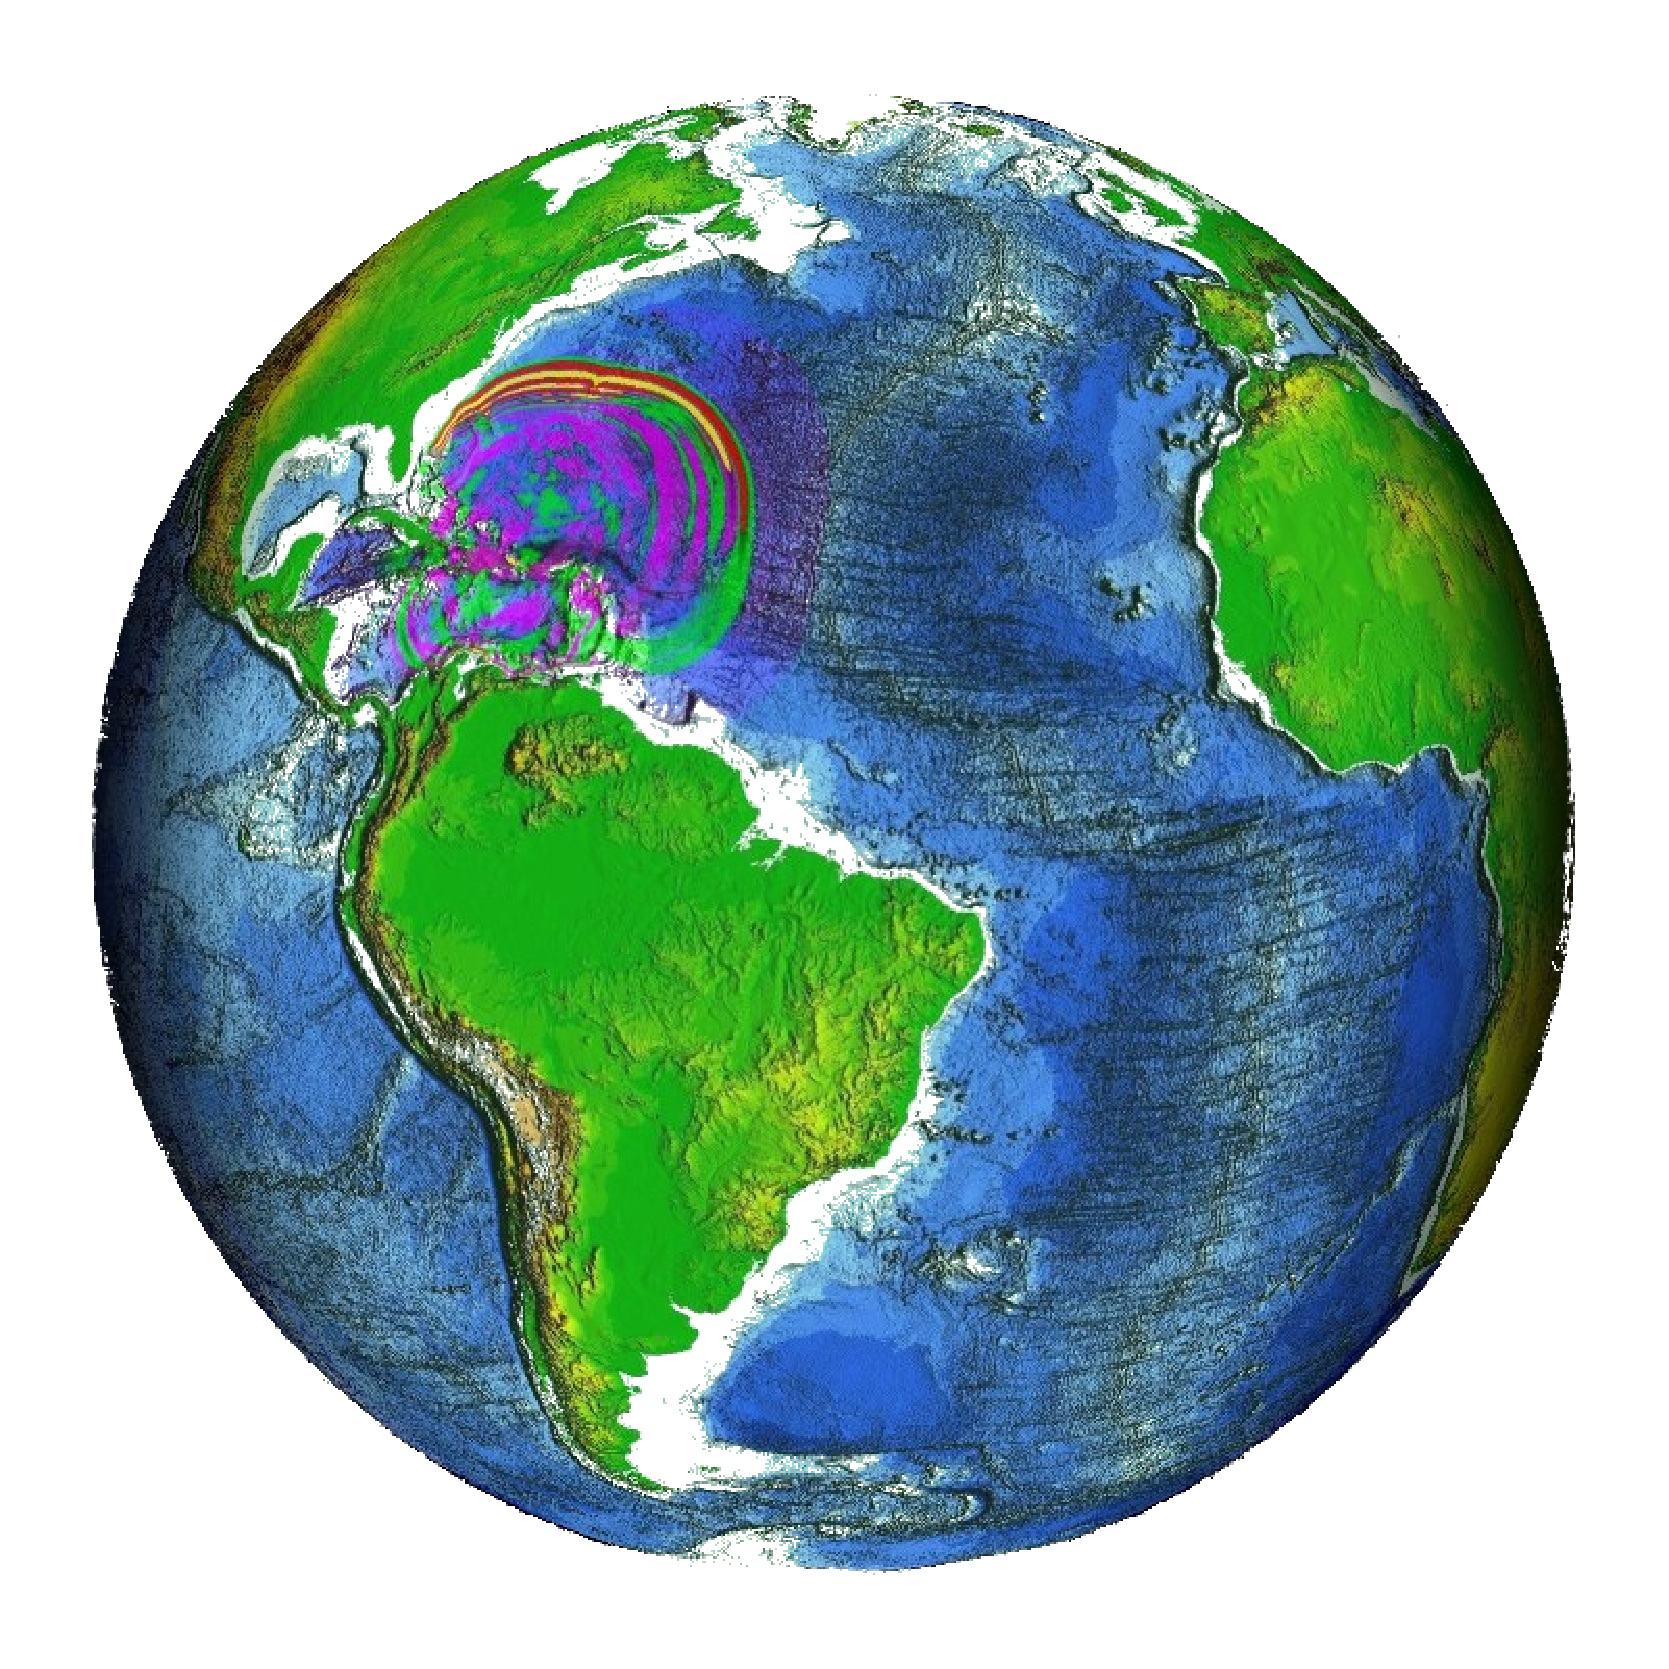
\includegraphics[scale=0.13]{globet.pdf}}}
	\put(80,7){\parbox[l]{12cm}{\Huge $\mathbf{\Rightarrow}$}}
	\put(105,-35){{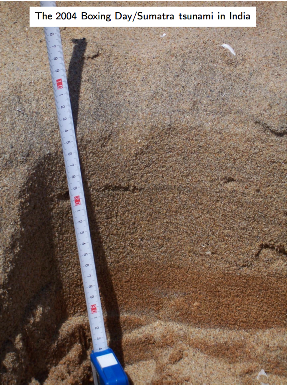
\includegraphics[scale=0.5]{tsunamisandindia.pdf}}}
	\put(175,7){\parbox[l]{12cm}{\Huge $\mathbf{\Rightarrow}$}}
	\put(200,-35){{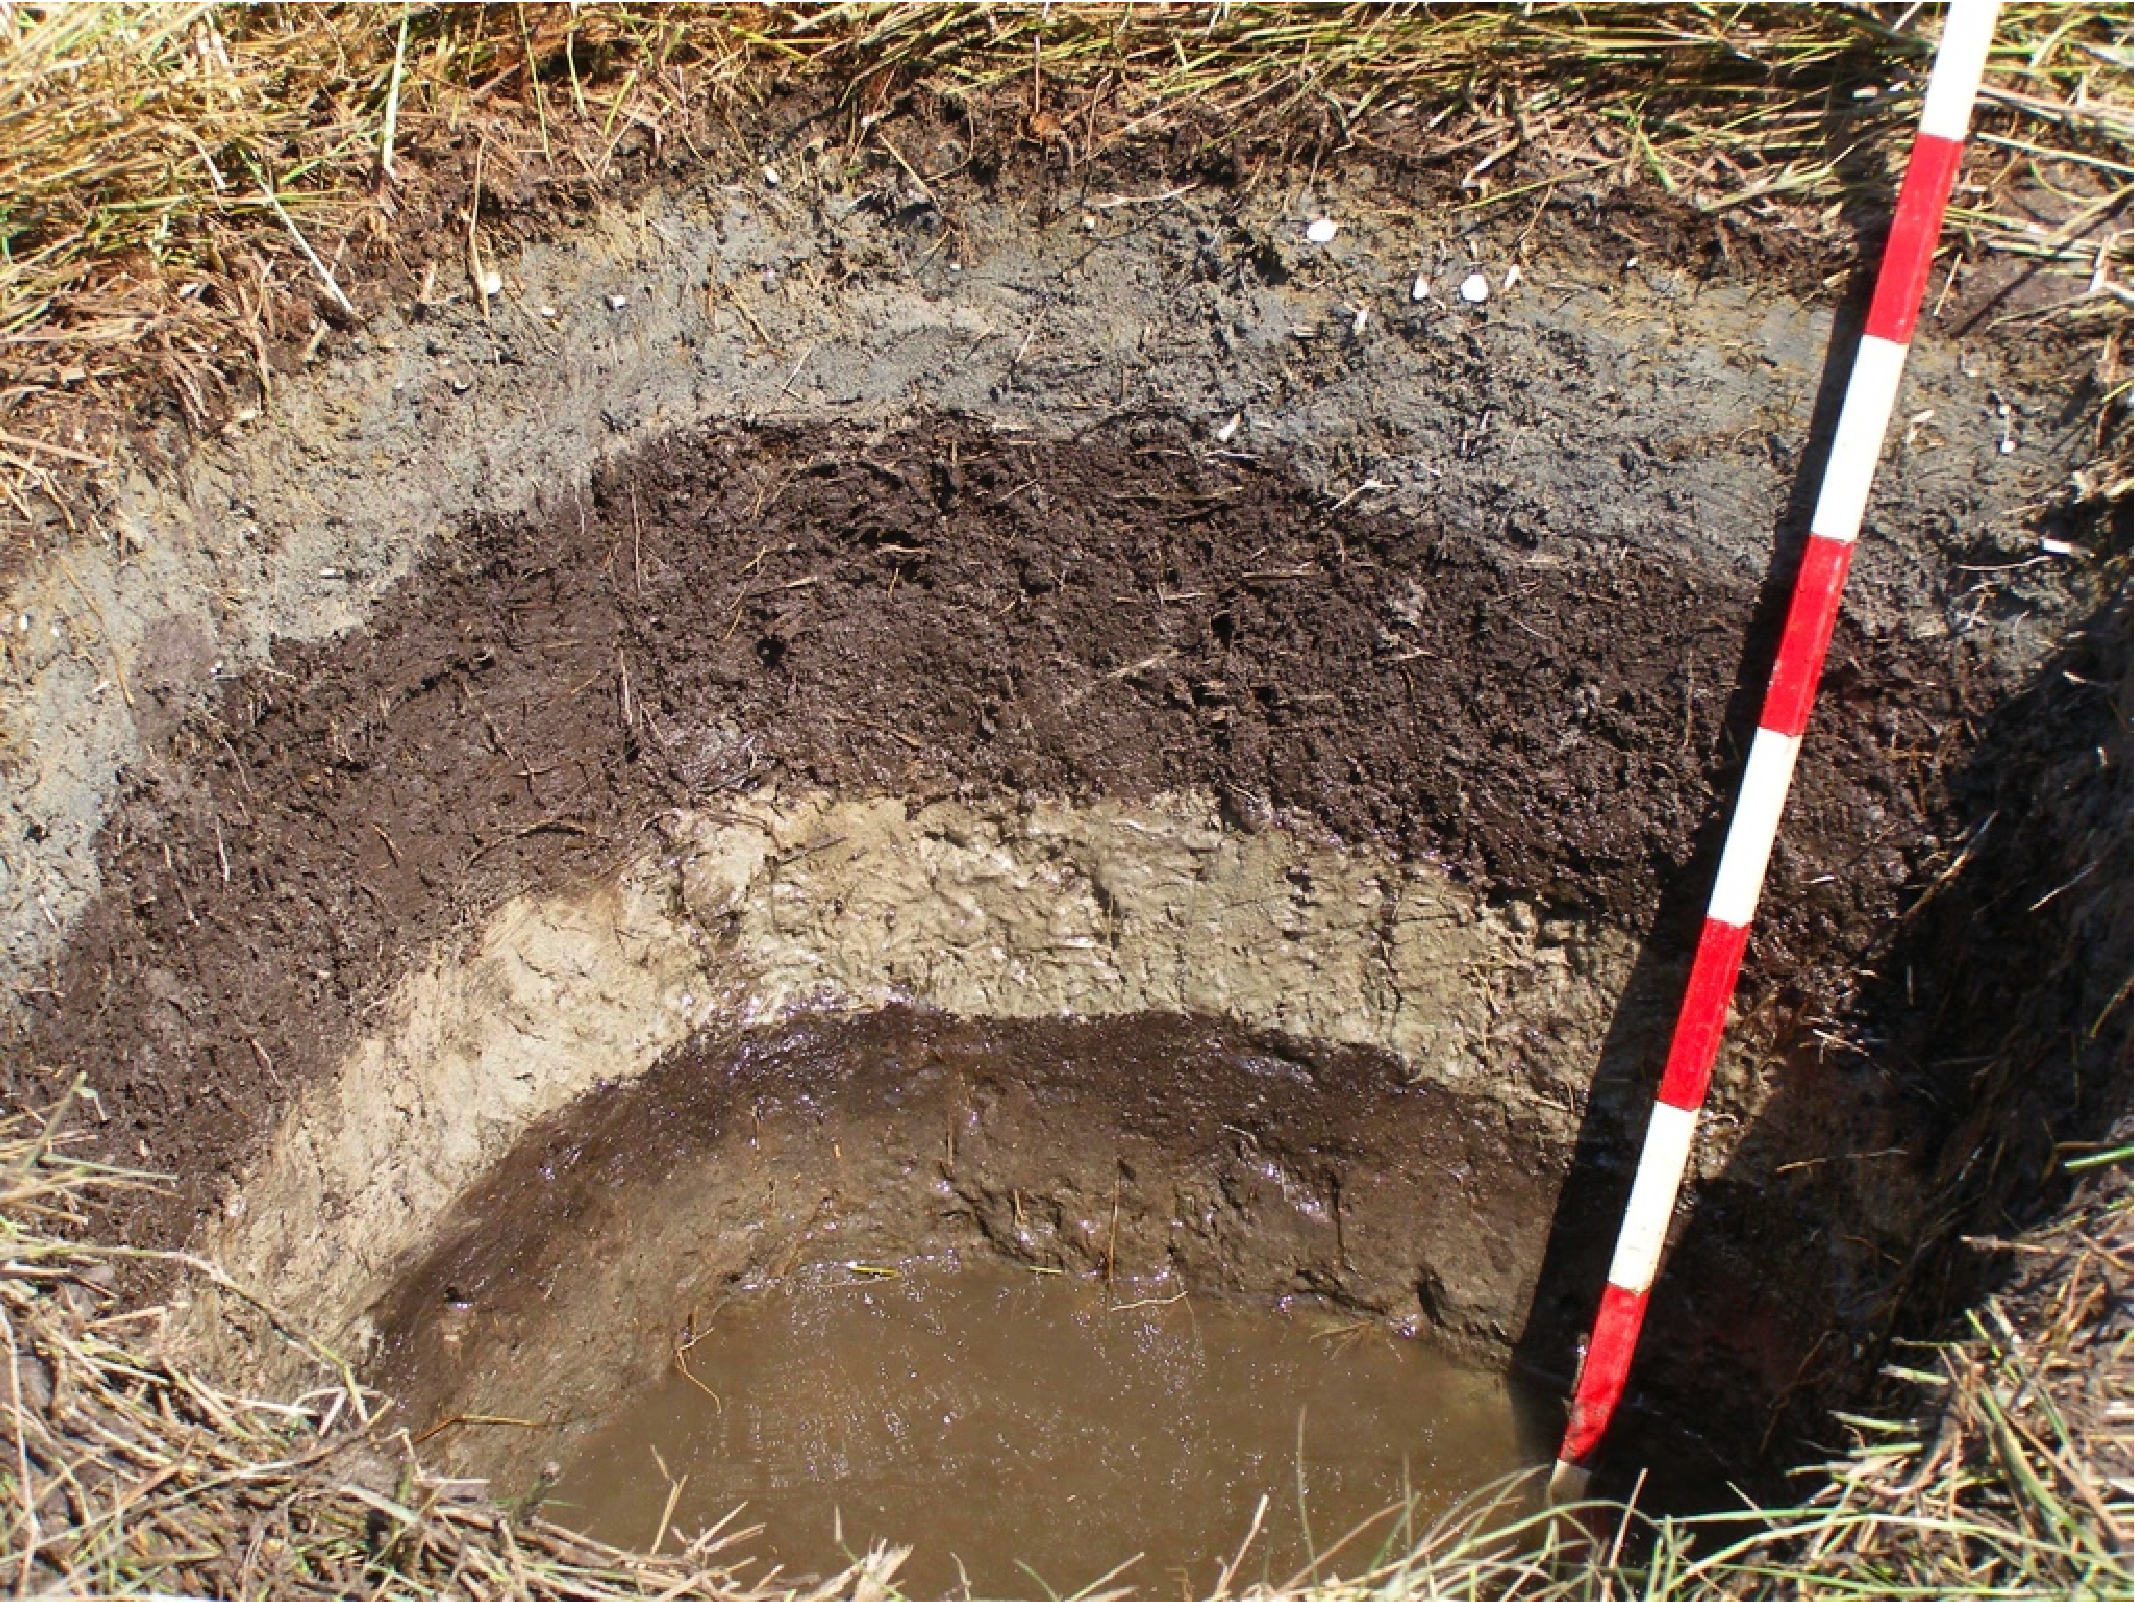
\includegraphics[scale=0.12]{tsunamisand.pdf}}}
%	\put(-27,-138){\parbox[l]{12cm}{\scriptsize Right picture: Thanks to Maria Beth Martin , University of Washington}}
	 \end{picture}
 \end{frame}

%  \begin{frame}[t]
%  \begin{center}
%    \vspace*{3.5em} 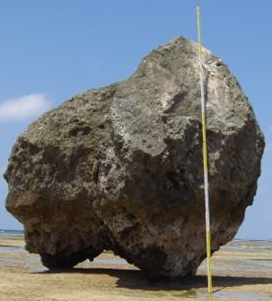
\includegraphics[scale=0.65]{boulderJapan.png} \\
%  \end{center}
%  \end{frame}
% 
\begin{frame}[c]
  \begin{center}
    {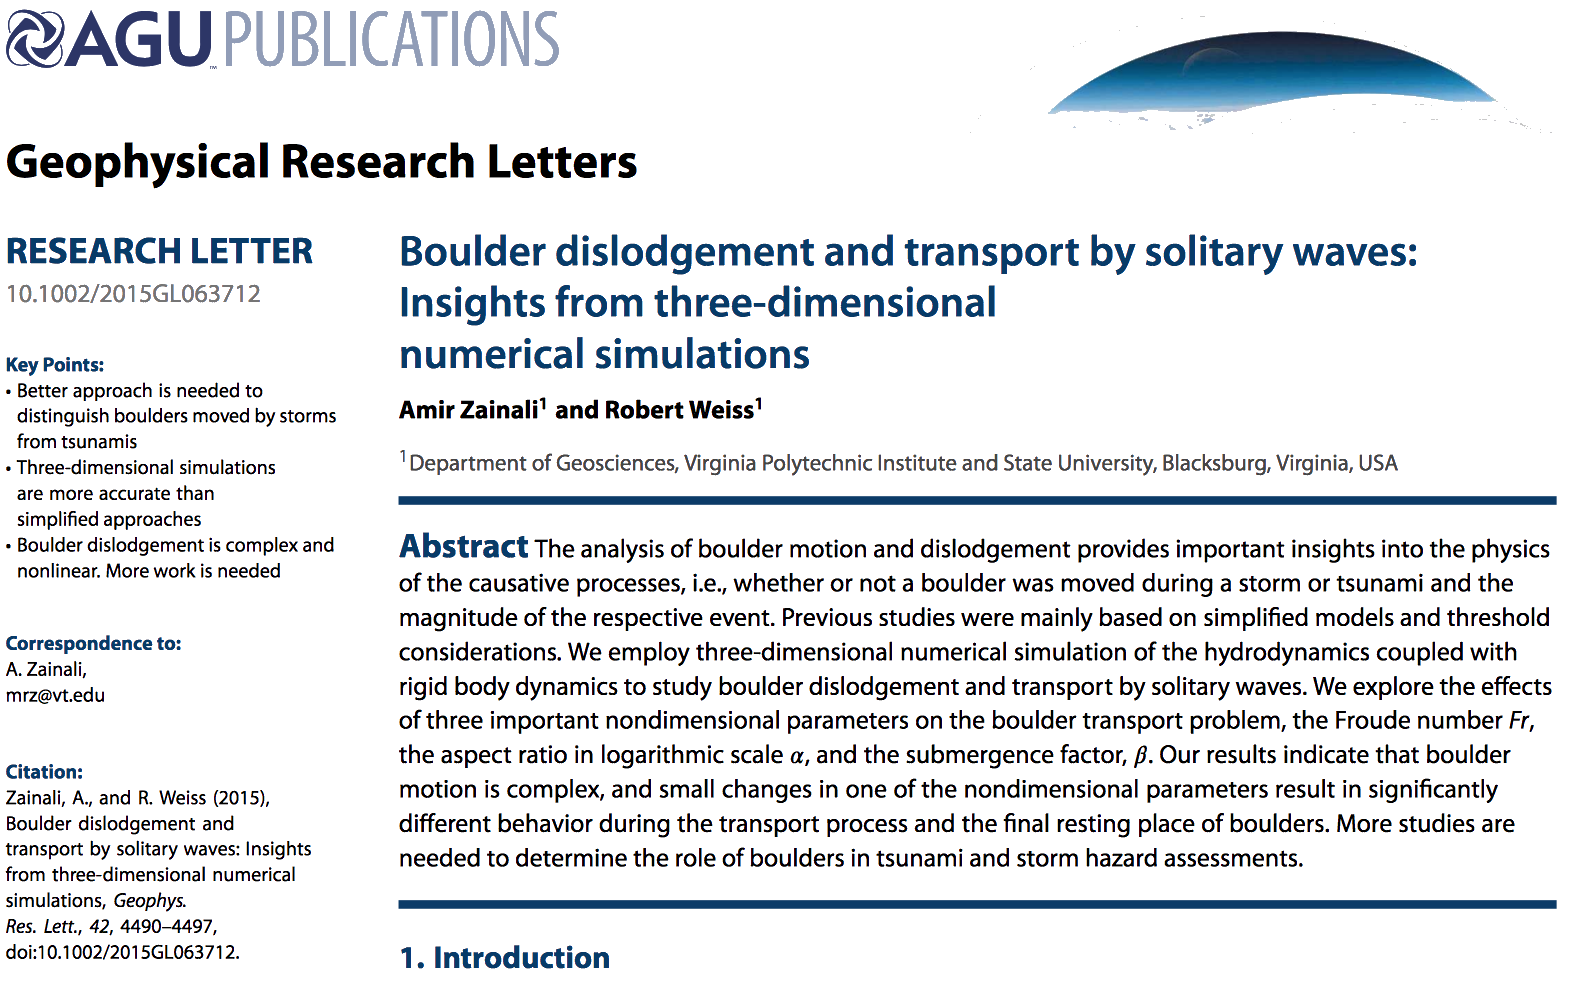
\includegraphics[scale=0.20]{threeDboulder1t.png}}
  \end{center}
\end{frame}

\begin{frame}[t]
\begin{center}
  \textbf{\Large Scaling Analysis}
\begin{eqnarray*}
    (h)_t + (uh)_x &=& 0 \\ \nonumber
    (hu)_t + (hu^2)_x + \frac{1}{2} (g h^2)_x &=& -g hb_x \nonumber
\end{eqnarray*}
\end{center}

   \only<2->{\begin{center}{\Huge $\Downarrow$}

\begin{eqnarray*}
    \mathrm{St}(h^*)_{t^*} + (u^*h^*)_{x^*} &=& 0 \\ \nonumber
    \mathrm{St}(h^*u^*)_{t^*} + (h*u^{*2})_{x^*} + \frac{1}{2\mathrm{Fr}^2} (h^{*2})_{x^*} &=& -\frac{\beta}{\mathrm{Fr}^2} h^* b^*_{x^*} \nonumber
\end{eqnarray*}
\end{center}

Strouhal number: $\mathrm{St} = \frac{x_{\mathrm{ref}}}{t_{\mathrm{ref}} u_{\mathrm{ref}}}$; Froude number: $\mathrm{Fr} = \frac{u_{\mathrm{ref}}}{\sqrt{g h_{\mathrm{ref}}}}$; Submergence: $\beta = \frac{b_{\mathrm{ref}}}{h_{\mathrm{ref}}}$. With $x_{\mathrm{ref}} = \kappa^{-1}$, $t_{\mathrm{ref}} = (c \kappa)^{-1}$, $h_{\mathrm{ref}} = h_w$, $u_{\mathrm{ref}} = c$, and $b_{\mathrm{ref}} = lb_y$, where $lb_y$ is boulder height, $c$ denotes wave speed, and $\kappa$ represents the wave number.}

\end{frame}

\begin{frame}[c]
  \begin{center}
  \hspace*{-0.5cm}  {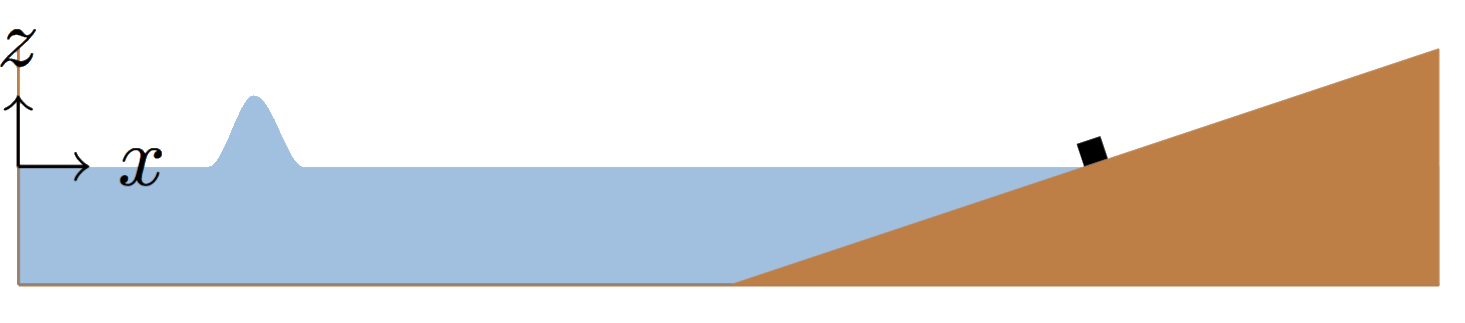
\includegraphics[scale=0.23]{3d_setupt.png}}
  \end{center}
\end{frame}

\begin{frame}[c]
  \begin{center}
  \hspace*{-0.5cm}  {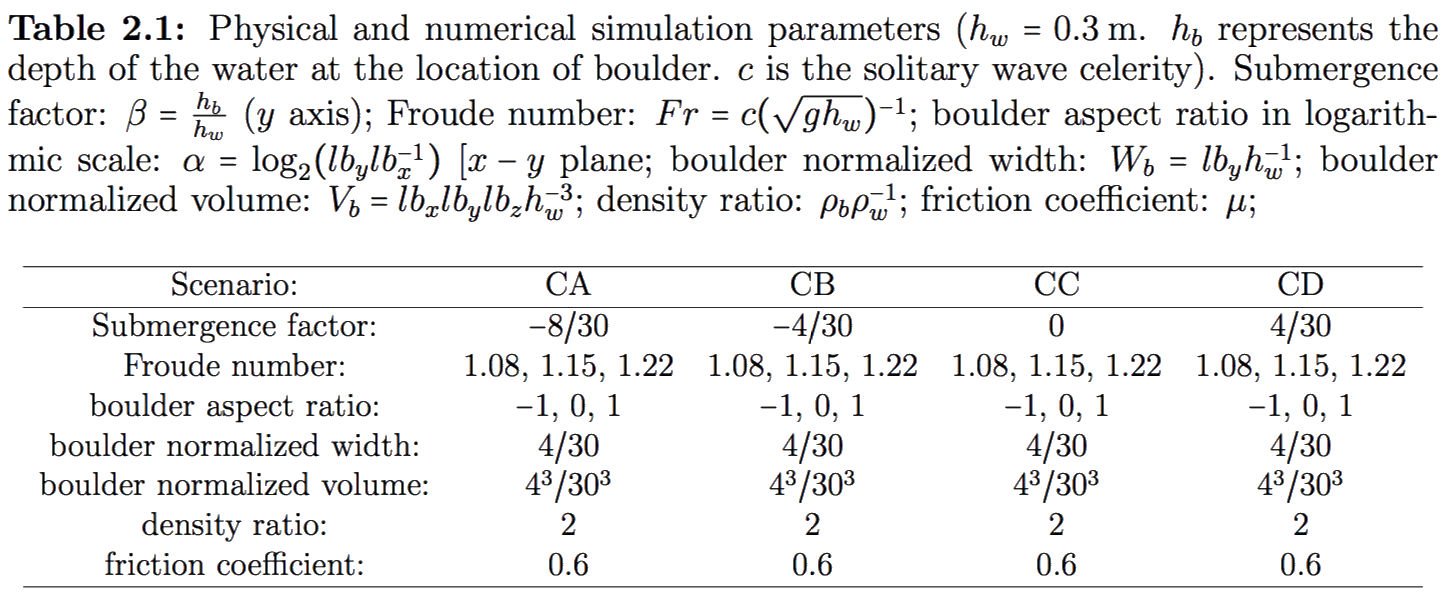
\includegraphics[scale=0.23]{3d_tablet.png}}
  \end{center}
\end{frame}

\begin{frame}[t]
  \begin{center}
  \vspace*{-0.5cm}\hspace*{-0.5cm}{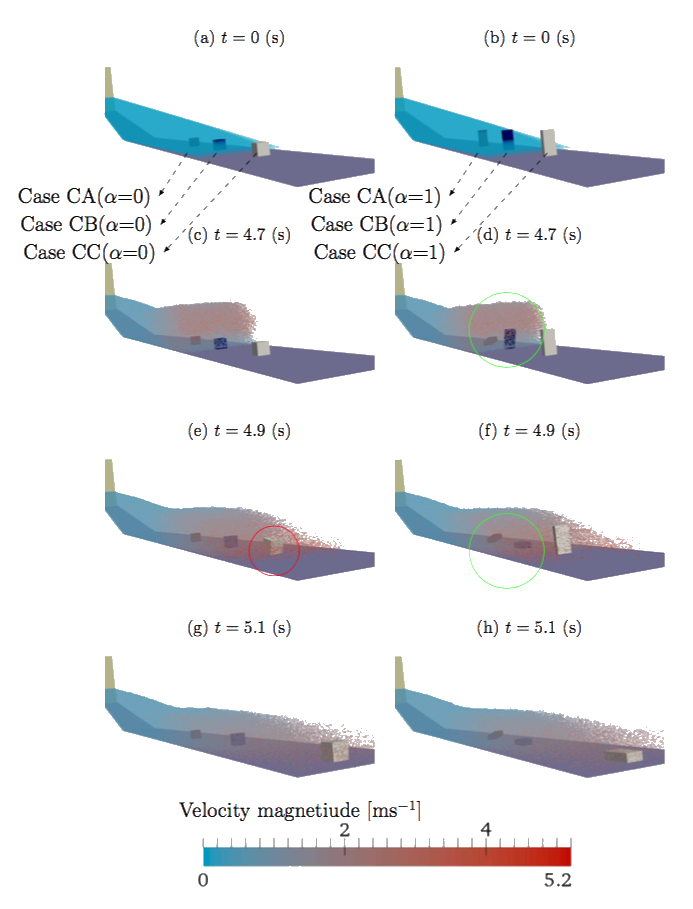
\includegraphics[scale=0.3]{3d_result1t.png}}
  \end{center}
\end{frame}

\begin{frame}[c]
  \begin{center}
  \vspace*{-0.25cm}\hspace*{-0.5cm}  {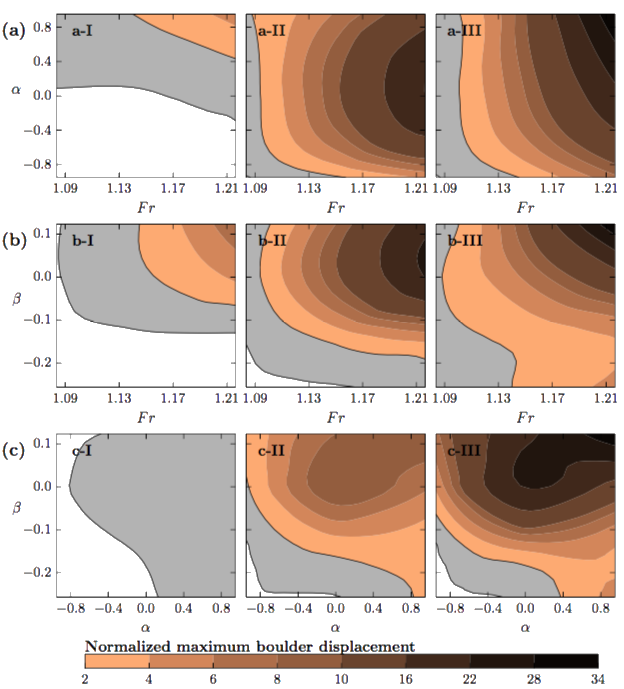
\includegraphics[scale=0.39]{3d_result2t.png}}
  \end{center}
\end{frame}


%%%%%######### Boulders #######################################################
\begin{frame}[fragile]%{Boulder Dislodgement}
%\topline
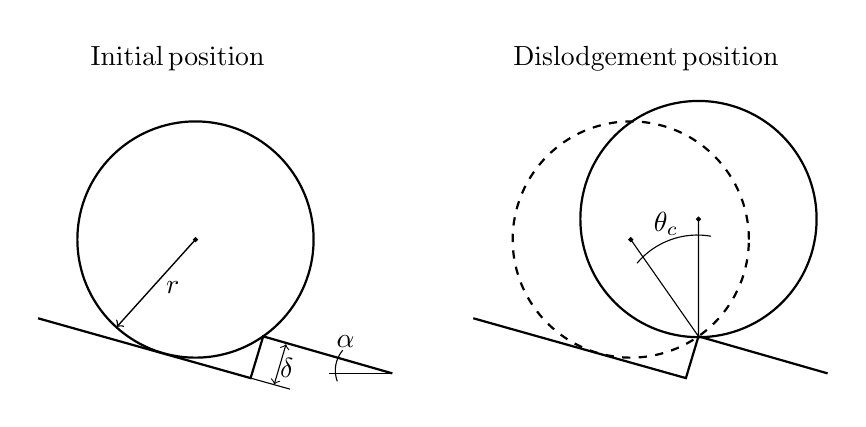
\begin{tikzpicture}
%%%left figure
\matrix[column sep=1cm] {
%%% (A)
\uncover<1->{
	\draw[line width=0.8pt] (0,0) circle (1.5cm);
%	\draw (0,0) circle (0.1cm);
	\filldraw (0, 0) circle (.025);
%	 \begin{scope}[style=axes]
	\draw[arrows=->,line width=.5pt]((0,0)--(-1,-1.11) node[right,xshift=0.5cm,yshift=0.5cm] {$r$};
	\draw[color=black] (1.,2.3) node[left] {$\mathrm{Initial\,position}$};

	\draw[line width=0.8pt]((-2.0,-1)--(0.7,-1.76)--(0.86,-1.23)-- (2.5,-1.7);

	\draw[line width=0.4pt]((0.7,-1.76)--(1.2,-1.9);
	\draw[arrows=<->,line width=.4pt]((1.0,-1.84)--(1.15,-1.33) node[right,xshift=-0.2cm,yshift=-0.3cm] {$\delta$};

	\draw[line width=0.4pt]((2.5,-1.7)--(1.7,-1.7);
	 \draw (1.8,-1.8) arc (200:140:0.4) node[right,xshift=-0.2cm,yshift=0.11cm] {$\alpha$};
     % \draw (15:2mm) node {$\alpha$};
     }
 \pgfmatrixnextcell
%%%(B)
\uncover<2->{
	\draw[dashed,line width=0.8pt] (0,0) circle (1.5cm);
	\filldraw (0, 0) circle (.025);


	\draw[line width=0.8pt] (0.86,0.26) circle (1.5cm);
	\filldraw (0.86, 0.26) circle (.025);
	\draw[line width=0.4pt]((0.86,0.26)--(0.86,-1.23)--(0,0);


	\draw[color=black] (2.,2.3) node[left] {$\mathrm{Dislodgement\,position}$};

	\draw[line width=0.8pt]((-2.0,-1)--(0.7,-1.76)--(0.86,-1.23)-- (2.5,-1.7);


	 \draw (0.08,-0.3) arc (140:80:1.0) node[right,xshift=-0.85cm,yshift=0.16cm] {$\theta_c$};
 	% \draw (15:2mm) node {$\alpha$};
    }
  \\
};
	\end{tikzpicture}

    \uncover<1->{$\alpha - \textrm{Slope}$, $\delta - \textrm{Roughness}$}

    \begin{center}
      \uncover<2->{$\theta_c(\delta, \alpha)=\left[{\frac{\pi}{2}} \delta - \alpha\right] \ge 0$}
    \end{center}
\end{frame}

\begin{frame}[t]%{Boulder Dislodgement}
%\topline
\uncover<1->{{\huge
\vspace{-1em}
\[
         \Sigma \mathbf{F} = \textrm{m} \mathbf{a}
        \]}}
 \uncover<2->{\Large \hspace{5cm}\reflectbox{\rotatebox[origin=c]{-90}{$\leadsto$} }\[(x,y) \rightarrow
 (\theta, r)\] \\ \hspace{5cm}\reflectbox{\rotatebox[origin=c]{-90}{$\leadsto$} } \\ \vspace{-0.3cm} {\huge \[
 \Sigma \mathbf{F} =\textrm{m}{\frac{\textrm{d}\theta^2}{\textrm{d} t^2}}=\textrm{m} \theta_{tt} \] }}

 \uncover<2->{with the assumption that $r = \textrm{const.}$}
\end{frame}


\begin{frame}[t]%{Boulder Dislodgement}
%\topline
This Equation of Motion can be rewritten [Schmeeckle and Nelson, 2003]:
$$
{\color{red} V\,L\ \left(\frac{7}{5}\rho_s+\rho_f C_m\right)}\theta_{tt}=\Sigma \mathbf{F}$$
\end{frame}

\begin{frame}[t]%{Boulder Dislodgement}
%\topline
This Equation of Motion can be rewritten [Schmeeckle and Nelson, 2003]:
$$
V\,L\ \left(\frac{7}{5}\rho_s+\rho_f C_m\right)\theta_{tt}={\color{red}\Sigma \mathbf{F}}$$

$$
{\color{red}\Sigma \mathbf{F}}=\mathbf{D}\sin{(\theta-\alpha)}+
(\mathbf{L}+\mathbf{B})\cos{(\theta -
\alpha)} - \mathbf{W}\cos{(\theta)}$$


With
\begin{itemize}
  \item[]$V$ -- particle volume, $\rho_s$ -- particle density, $\rho_f$ -- fluid density,
  \item[]$L$ -- distance between the center of gravity and point of rotation ($r$),
  \item[]$C_m$ -- added mass coefficient (0.5 for spheres in water),
  \item[]$\mathbf{D}$ -- drag, $\mathbf{L}$ -- lift, $\mathbf{B}$ -- buoyancy, $\mathbf{W}$ -- weight
\end{itemize}

\end{frame}


%\begin{frame}[t]{Boulder Transport -- Waves}
%  \topline
%  {\bf  Assumptions:}
%    \begin{itemize}
%      \item Fully submerged, spherical boulders
%      \item Depth-limited, linear, shallow water, waves
%    \end{itemize}
%    \begin{picture}(1,6)
%  \put(-20,-170){ \includegraphics[scale=0.47]{shallowwater.png}}
%  \put(120,-10){ Relationship between velocity and }
%  \put(120,-20){ amplitude: }
%  \put(180, -50){$A=\frac{u_o\,d}{\sqrt{g\,d}}$
%}
% \end{picture}
%\end{frame}




%\begin{frame}{Particle Transport -- Boulders}
%  \topline
%
%{\bf Relationship} between amplitude ($A$) and veloctiy ($u_o$):
%\vspace{-0.6em}
%\[
%A=\frac{u_o\,d}{\sqrt{g\,d}}
%\]
%
%{\bf Wave time series:}
%
%\begin{eqnarray}
%u(t)=u_o\,\sin{\left(\frac{2\pi\,t}{T}\right)} \nonumber \\ \nonumber
%\eta(t)=A\,\sin{\left(\frac{2\pi\,t}{T}\right)}
%\end{eqnarray}
%($T$ -- Wave period)
%\end{frame}

\begin{frame}[c]%{Boulder Dislodgement}
%\topline
  Example: $\alpha=0$ and $\delta=1$ $\leadsto\; \theta_c=0.5\pi$
  \begin{center}
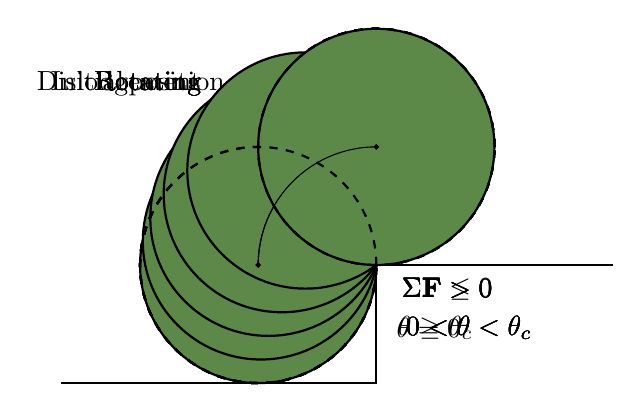
\begin{tikzpicture}
	\uncover<1>{\draw[line width=0.8pt,fill=Fern] (-2,-2) circle (1.5cm);
	\filldraw (-2, -2) circle (.025);
	\draw[line width=0.8pt]((-4.5,-3.5)--(-0.5,-3.5)--(-0.5,-2)-- (2.5,-2);
    \draw[dashed, line width=0.8pt] (-0.5,-0.5) circle (1.5cm);
    \filldraw (-0.5, -0.5) circle (.025);
	\draw (-0.5,-0.5) arc (270:360:-1.5) node[right,pos=0.5]{};
	\draw[color=black] (-2.3,.3) node[left] {$\textrm{Initial\,position}$};
    \draw[color=black] (1.1,-2.3) node[left] {$\Sigma \mathbf{F}\le 0$};
    \draw[color=black] (0.7,-2.8) node[left] {$\theta = 0$};
    }

 \uncover<2>{
    \draw[line width=0.8pt,fill=Fern] (-1.965,-1.7) circle (1.5cm);
	\filldraw (-1.965, -1.7) circle (.025);
    \draw[dashed,line width=0.8pt] (-2,-2) circle (1.5cm);
	\filldraw (-2, -2) circle (.025);
	\draw[line width=0.8pt]((-4.5,-3.5)--(-0.5,-3.5)--(-0.5,-2)-- (2.5,-2);
    \draw[dashed, line width=0.8pt] (-0.5,-0.5) circle (1.5cm);
	\draw (-0.5,-0.5) arc (270:360:-1.5) node[right,pos=0.5]{};
    \filldraw (-0.5, -0.5) circle (.025);
    \draw[color=black] (-2.6,.3) node[left] {$\textrm{Rotating}$};
    \draw[color=black] (1.1,-2.3) node[left] {$\Sigma \mathbf{F} > 0$};
    \draw[color=black] (1.6,-2.8) node[left] {$0<\theta <\theta_c$};
    }

 \uncover<3>{
    \draw[line width=0.8pt,fill=Fern] (-1.87,-1.4) circle (1.5cm);
	\filldraw (-1.87, -1.4) circle (.025);
    \draw[dashed,line width=0.8pt] (-2,-2) circle (1.5cm);
	\filldraw (-2, -2) circle (.025);
	\draw[line width=0.8pt]((-4.5,-3.5)--(-0.5,-3.5)--(-0.5,-2)-- (2.5,-2);
    \draw[dashed, line width=0.8pt] (-0.5,-0.5) circle (1.5cm);
	\draw (-0.5,-0.5) arc (270:360:-1.5) node[right,pos=0.5]{};
    \filldraw (-0.5, -0.5) circle (.025);
    \draw[color=black] (-2.6,.3) node[left] {$\textrm{Rotating}$};
    \draw[color=black] (1.1,-2.3) node[left] {$\Sigma \mathbf{F} > 0$};
    \draw[color=black] (1.6,-2.8) node[left] {$0<\theta <\theta_c$};
    }

  \uncover<4>{
    \draw[line width=0.8pt,fill=Fern] (-1.7,-1.1) circle (1.5cm);
	\filldraw (-1.7, -1.1) circle (.025);
    \draw[dashed,line width=0.8pt] (-2,-2) circle (1.5cm);
	\filldraw (-2, -2) circle (.025);
	\draw[line width=0.8pt]((-4.5,-3.5)--(-0.5,-3.5)--(-0.5,-2)-- (2.5,-2);
    \draw[dashed, line width=0.8pt] (-0.5,-0.5) circle (1.5cm);
	\draw (-0.5,-0.5) arc (270:360:-1.5) node[right,pos=0.5]{};
    \filldraw (-0.5, -0.5) circle (.025);
    \draw[color=black] (-2.6,.3) node[left] {$\textrm{Rotating}$};
    \draw[color=black] (1.1,-2.3) node[left] {$\Sigma \mathbf{F} > 0$};
    \draw[color=black] (1.6,-2.8) node[left] {$0<\theta <\theta_c$};
    }

   \uncover<5>{
    \draw[line width=0.8pt,fill=Fern] (-1.4,-0.8) circle (1.5cm);
	\filldraw (-1.40, -0.8) circle (.025);
    \draw[dashed,line width=0.8pt] (-2,-2) circle (1.5cm);
	\filldraw (-2, -2) circle (.025);
	\draw[line width=0.8pt]((-4.5,-3.5)--(-0.5,-3.5)--(-0.5,-2)-- (2.5,-2);
    \draw[dashed, line width=0.8pt] (-0.5,-0.5) circle (1.5cm);
	\draw (-0.5,-0.5) arc (270:360:-1.5) node[right,pos=0.5]{};
    \filldraw (-0.5, -0.5) circle (.025);
    \draw[color=black] (-2.6,.3) node[left] {$\textrm{Rotating}$};
    \draw[color=black] (1.6,-2.8) node[left] {$0<\theta <\theta_c$};
    \draw[color=black] (1.1,-2.3) node[left] {$\Sigma \mathbf{F} > 0$};
    }

   \uncover<6->{
    \draw[line width=0.8pt,fill=Fern] (-0.5,-0.5) circle (1.5cm);
	\filldraw (-0.5, -0.5) circle (.025);
    \draw[dashed,line width=0.8pt] (-2,-2) circle (1.5cm);
	\filldraw (-2, -2) circle (.025);
	\draw[line width=0.8pt]((-4.5,-3.5)--(-0.5,-3.5)--(-0.5,-2)-- (2.5,-2);
    \draw[dashed, line width=0.8pt] (-0.5,-0.5) circle (1.5cm);
	\draw (-0.5,-0.5) arc (270:360:-1.5) node[right,pos=0.5]{};
    \filldraw (-0.5, -0.5) circle (.025);
    \draw[color=black] (-2.6,.3) node[left] {$\textrm{Dislodgement}$};
    \draw[color=black] (0.85,-2.8) node[left] {$\theta \ge \theta_c$};
    \draw[color=black] (1.1,-2.3) node[left] {$\Sigma \mathbf{F} > 0$};
    }
  \end{tikzpicture}

  \uncover<6->{Duration of rotation: $T_r = t(\textrm{for\,}\theta = \theta_c)-t(\textrm{for\,} \Sigma
  \mathrm{F}=0) $}

  \uncover<7->{$$I=\int\limits_{t_o}^{t_o+T_r}\!\!\!\!\!\Sigma \mathbf{F} \mathbf{d}\textrm{t} \ge I_c$$ }
    \end{center}
\end{frame}

% \begin{frame}[t]{Boulder Dislodgement}
% \topline
% Why Version 1.0:

% \begin{center}

% \vspace{-0.2cm}\includegraphics[scale=0.45]{singlewave.jpg}
% \end{center}
% \end{frame}

% \begin{frame}[t]{Boulder Dislodgement}
% \topline
% \begin{center}
% Version 1.0 $\Rightarrow$ Version 2.0

% %\vspace{0.2cm}
% \only<1>{\vspace{0.2cm}\includegraphics[scale=0.42]{fig2.jpg}}

% \only<2>{\vspace{0.2cm}\includegraphics[scale=0.27]{wave1.jpg}}

% \only<3>{\vspace{0.2cm}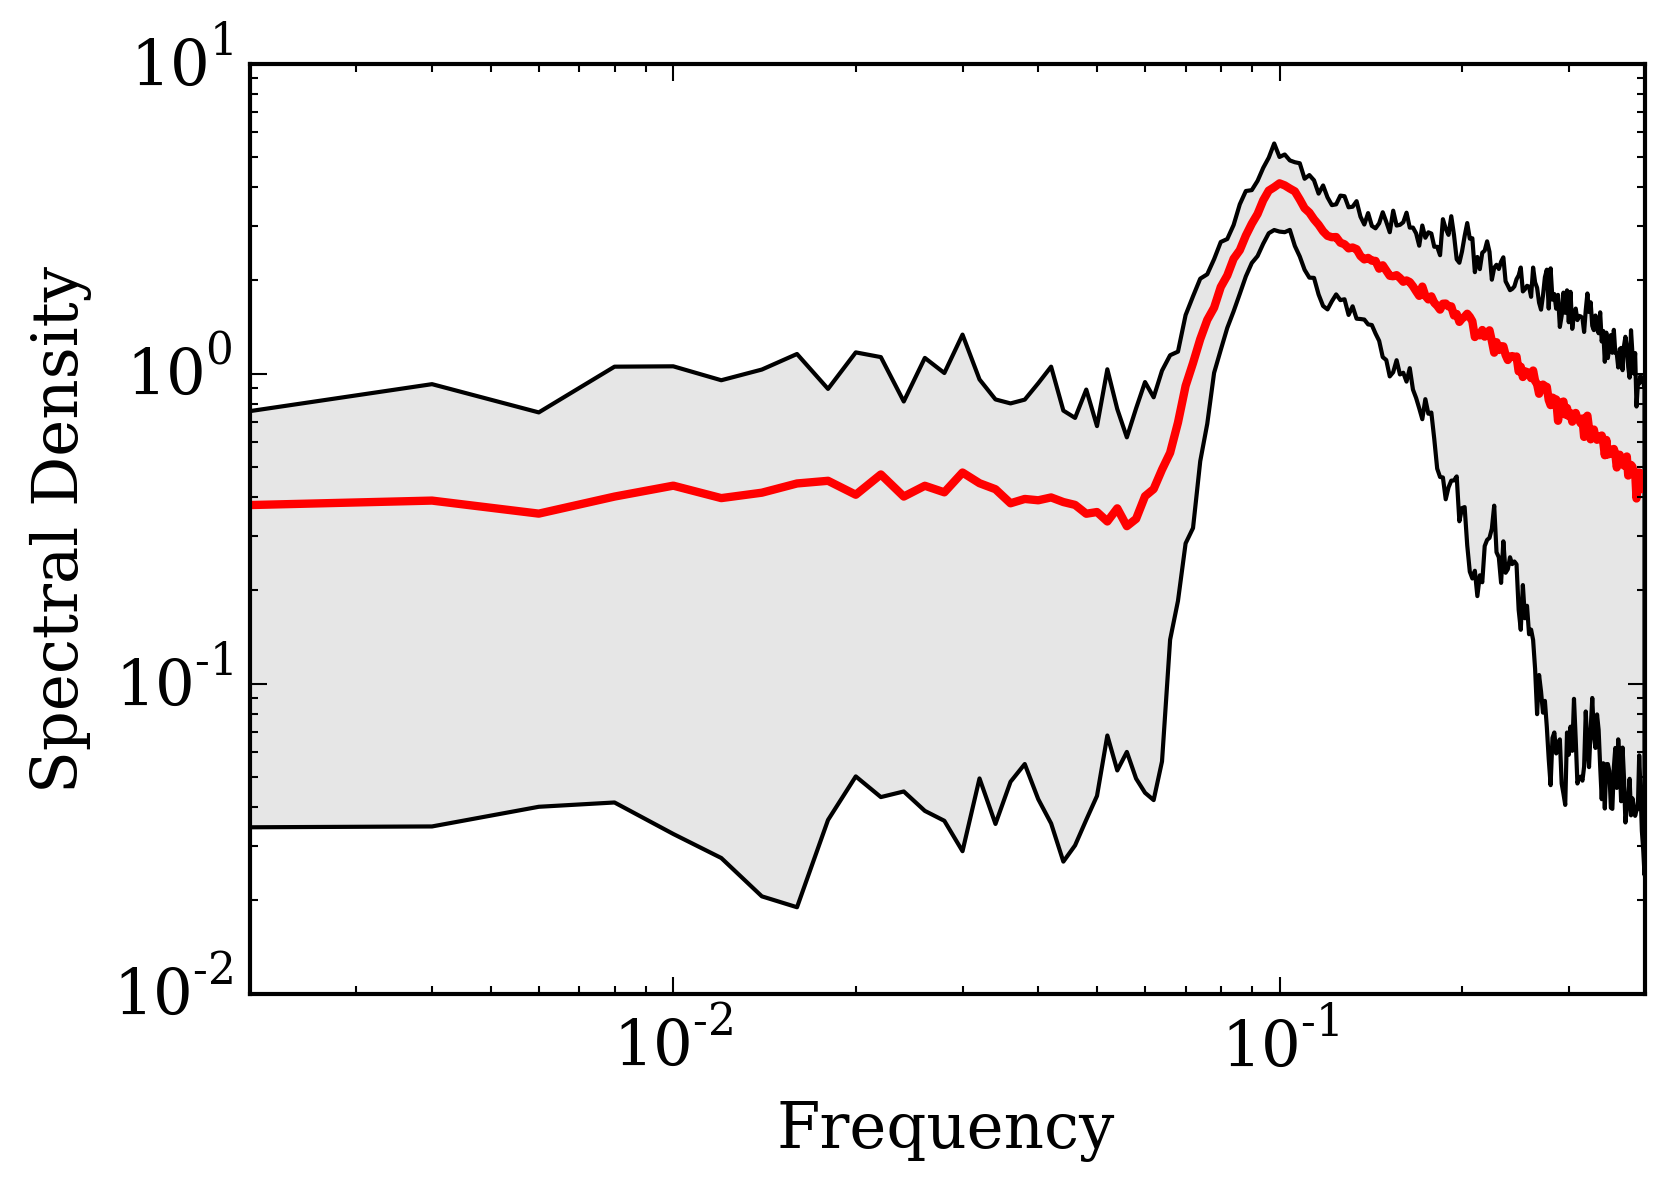
\includegraphics[scale=0.67]{fig6.png}}
% \end{center}
% \end{frame}


\begin{frame}[c]%{Boulder Dislodgement}
\begin{center}
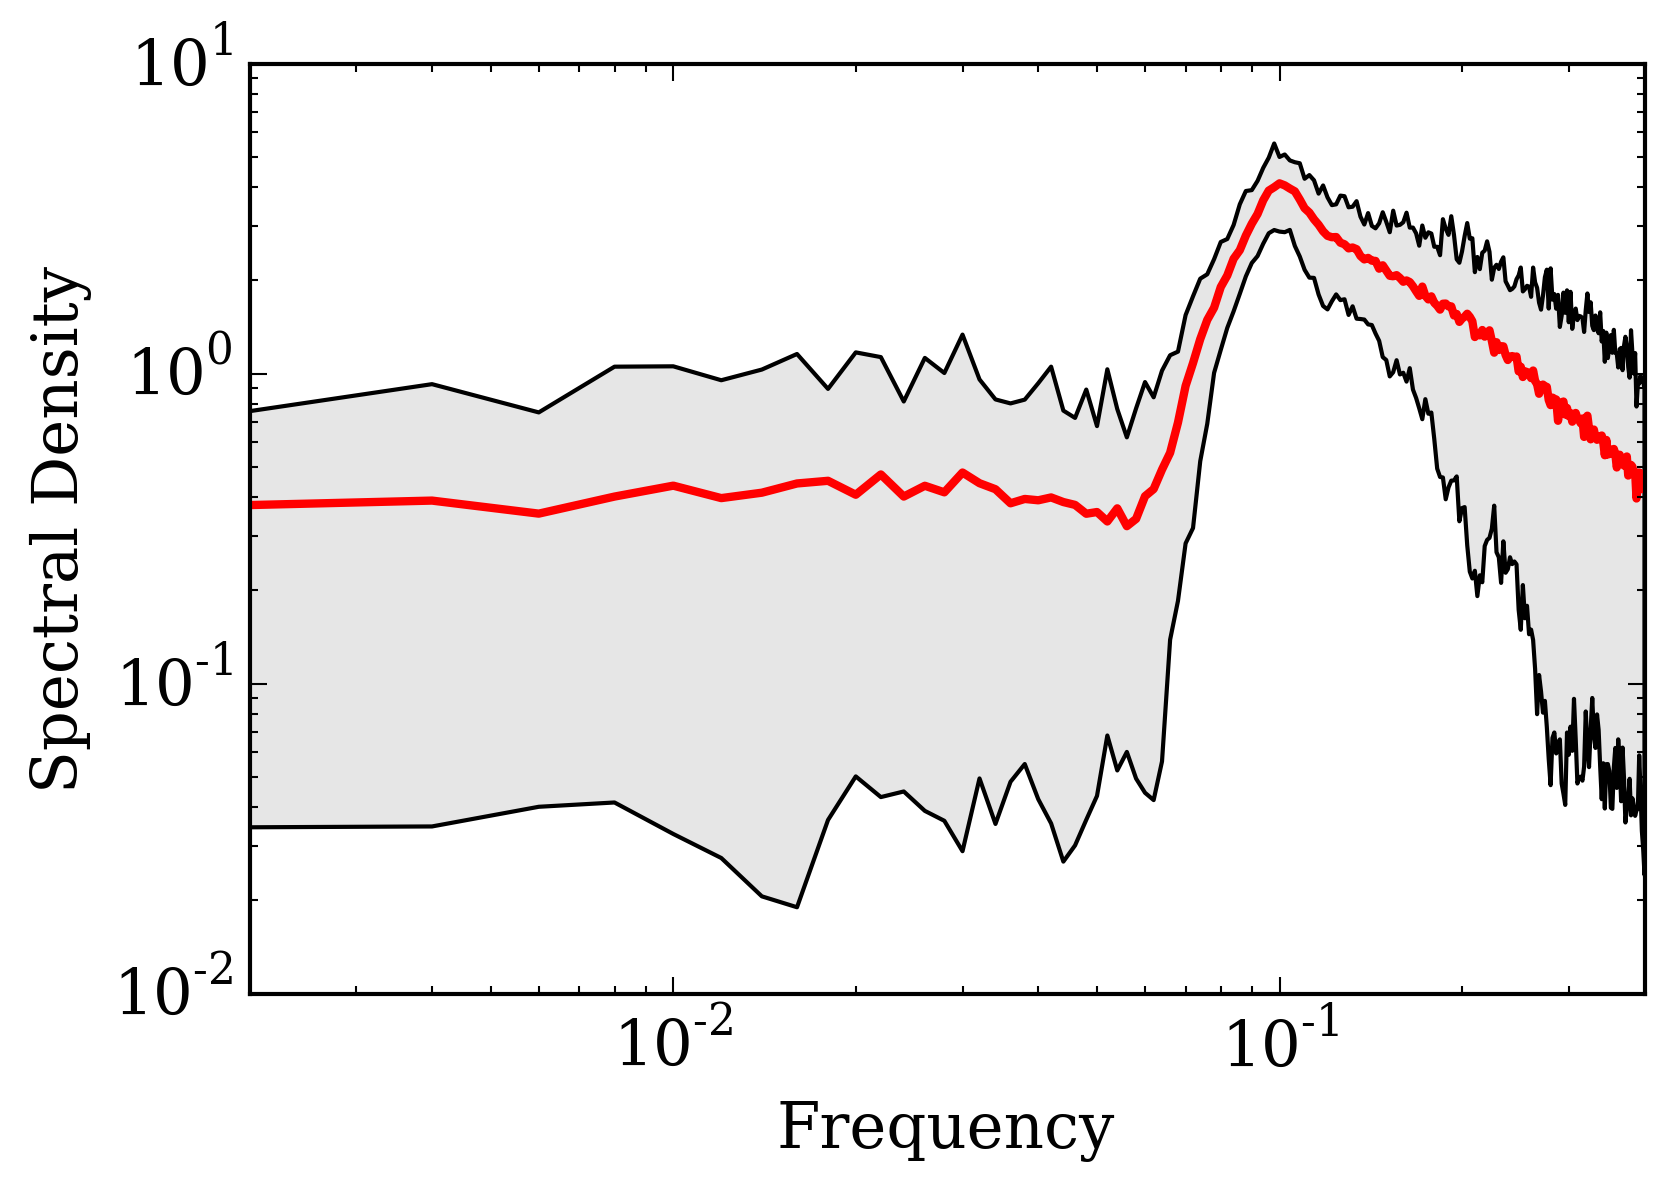
\includegraphics[scale=0.8]{fig6t.png}
\end{center}
\end{frame}

\begin{frame}[c]%{Boulder Dislodgement}

\begin{center}

\vspace{0.5cm}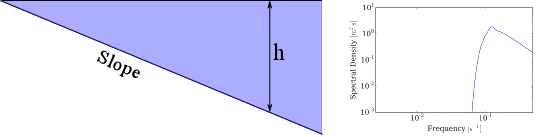
\includegraphics[scale=0.5]{modelt.png}
\end{center}


  \begin{multline}
\frac{db_{J}}{dx}=-i\sum_{\begin{array}{c}
P,Q\end{array}}W_{J,\pm P,Q}b_{P}b_{Q}e^{-i\Delta_{J,P,Q}\theta}\delta_{J,Q+P} \\ +2i\sum_{\begin{array}{c}
P,Q\end{array}}W_{J,\pm P,Q}b_{-P}b_{Q}e^{-i\Delta_{J,-P,Q}\theta}\delta_{J,Q-P}.\label{eq: triads}
\end{multline}
\end{frame}

\begin{frame}[t]%{Boulder Dislodgement}
\begin{center}
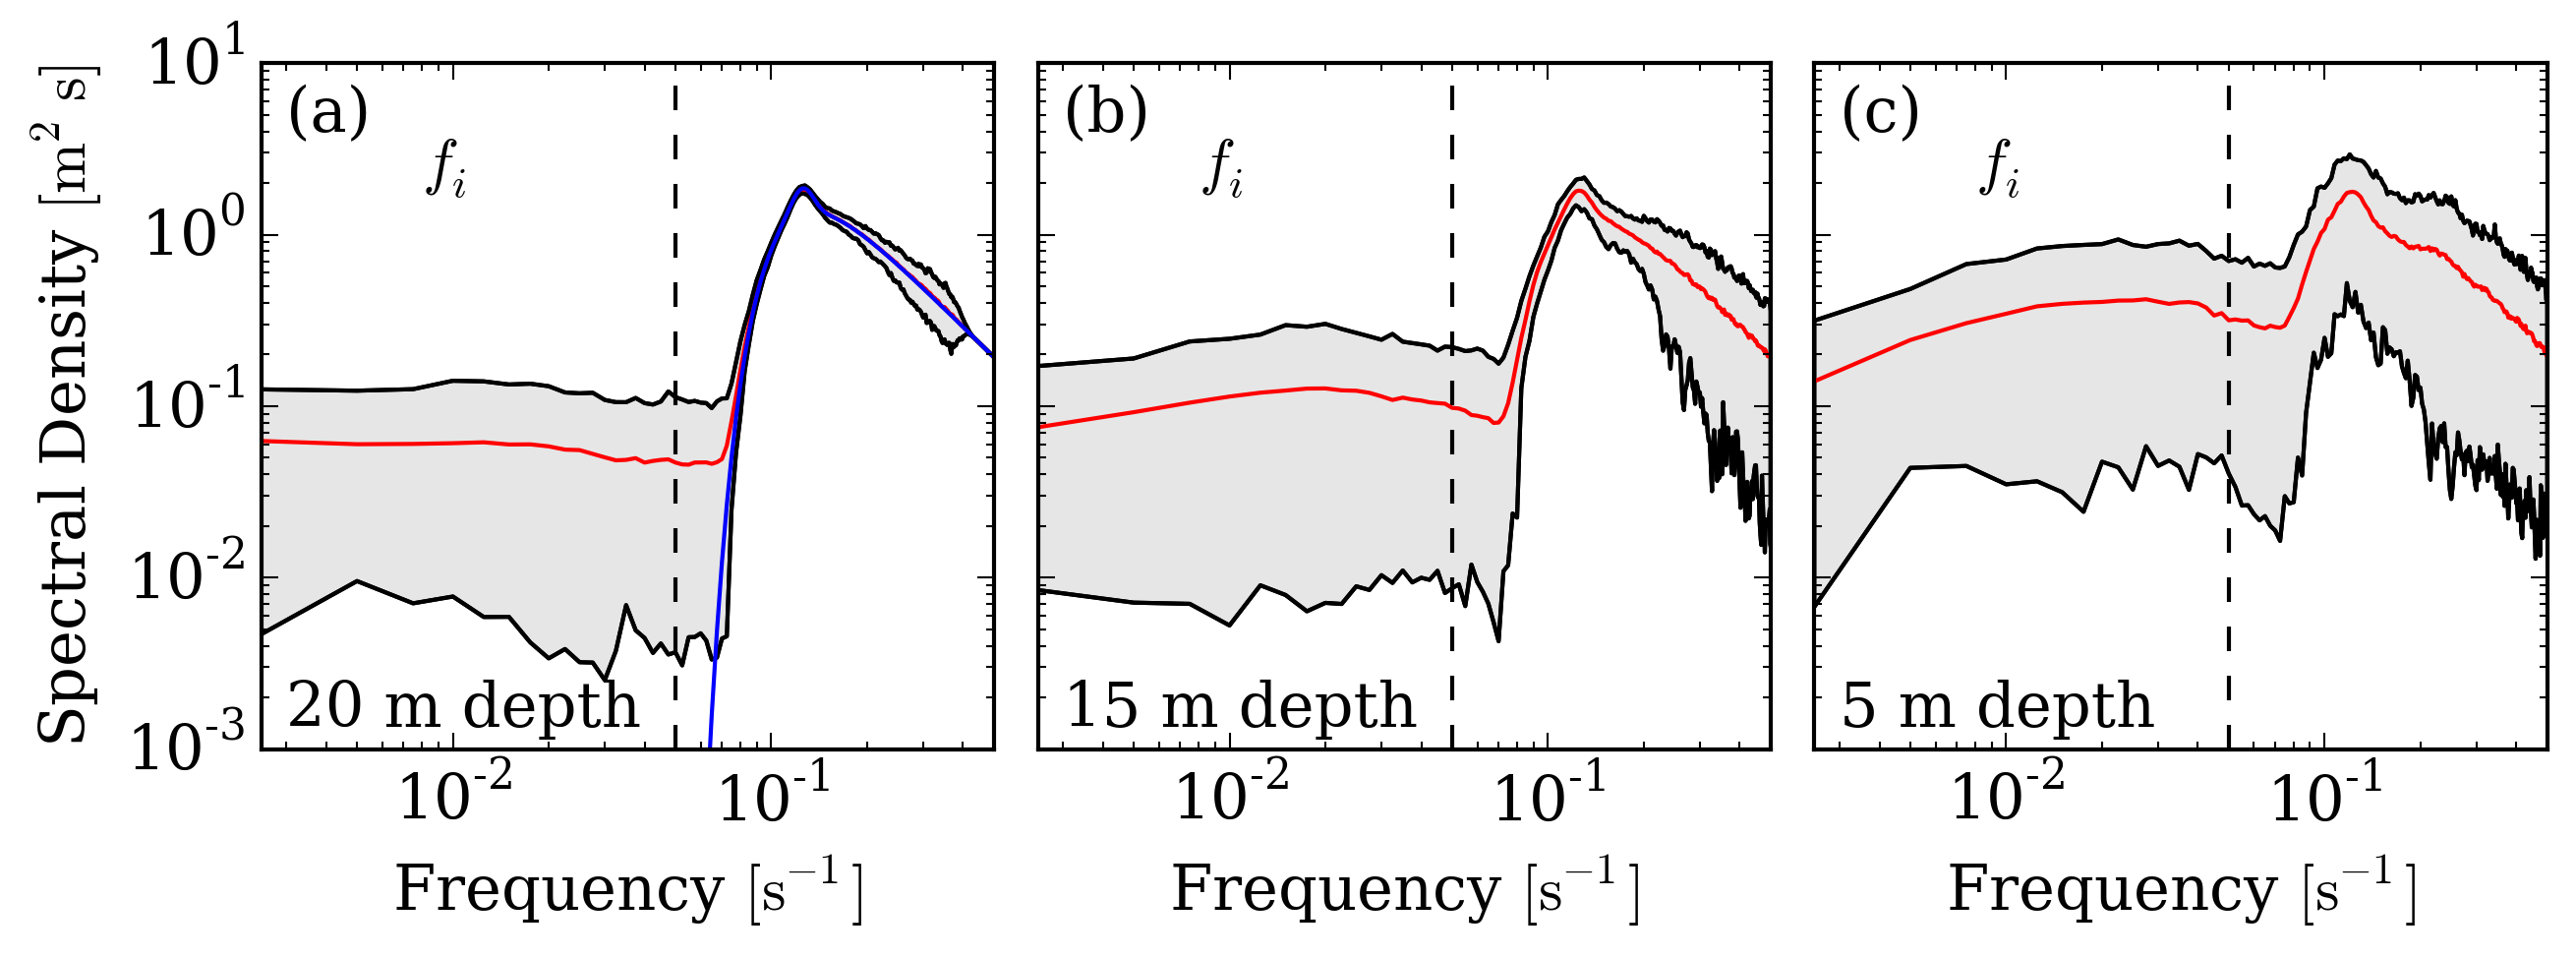
\includegraphics[scale=0.47]{FigRiset.png}

\begin{equation}
\tilde{E}=\frac{\int_{f>0.05}(\textrm{Spectral Density})}{\int_{f}(\textrm{Spectral Density})} \nonumber
\end{equation}
$\tilde{E}_{(a)} = 5.6\times 10^{-4}$, $\tilde{E}_{(b)} = 2.3\times10^{-3}$, $\tilde{E}_{(c)} = 2.6\times 10^{-2}$
\end{center}
\end{frame}

% \begin{frame}[c]{Boulder Dislodgement: Version 2.0}
% \topline
% \vspace{-0.5cm}
% \begin{center}
% \includegraphics[scale=0.35]{EnergyRatioSlopes1.png}
% \end{center}
% \end{frame}


\begin{frame}[c]%{Boulder Dislodgement}
\vspace{-0.75cm}
\begin{center}
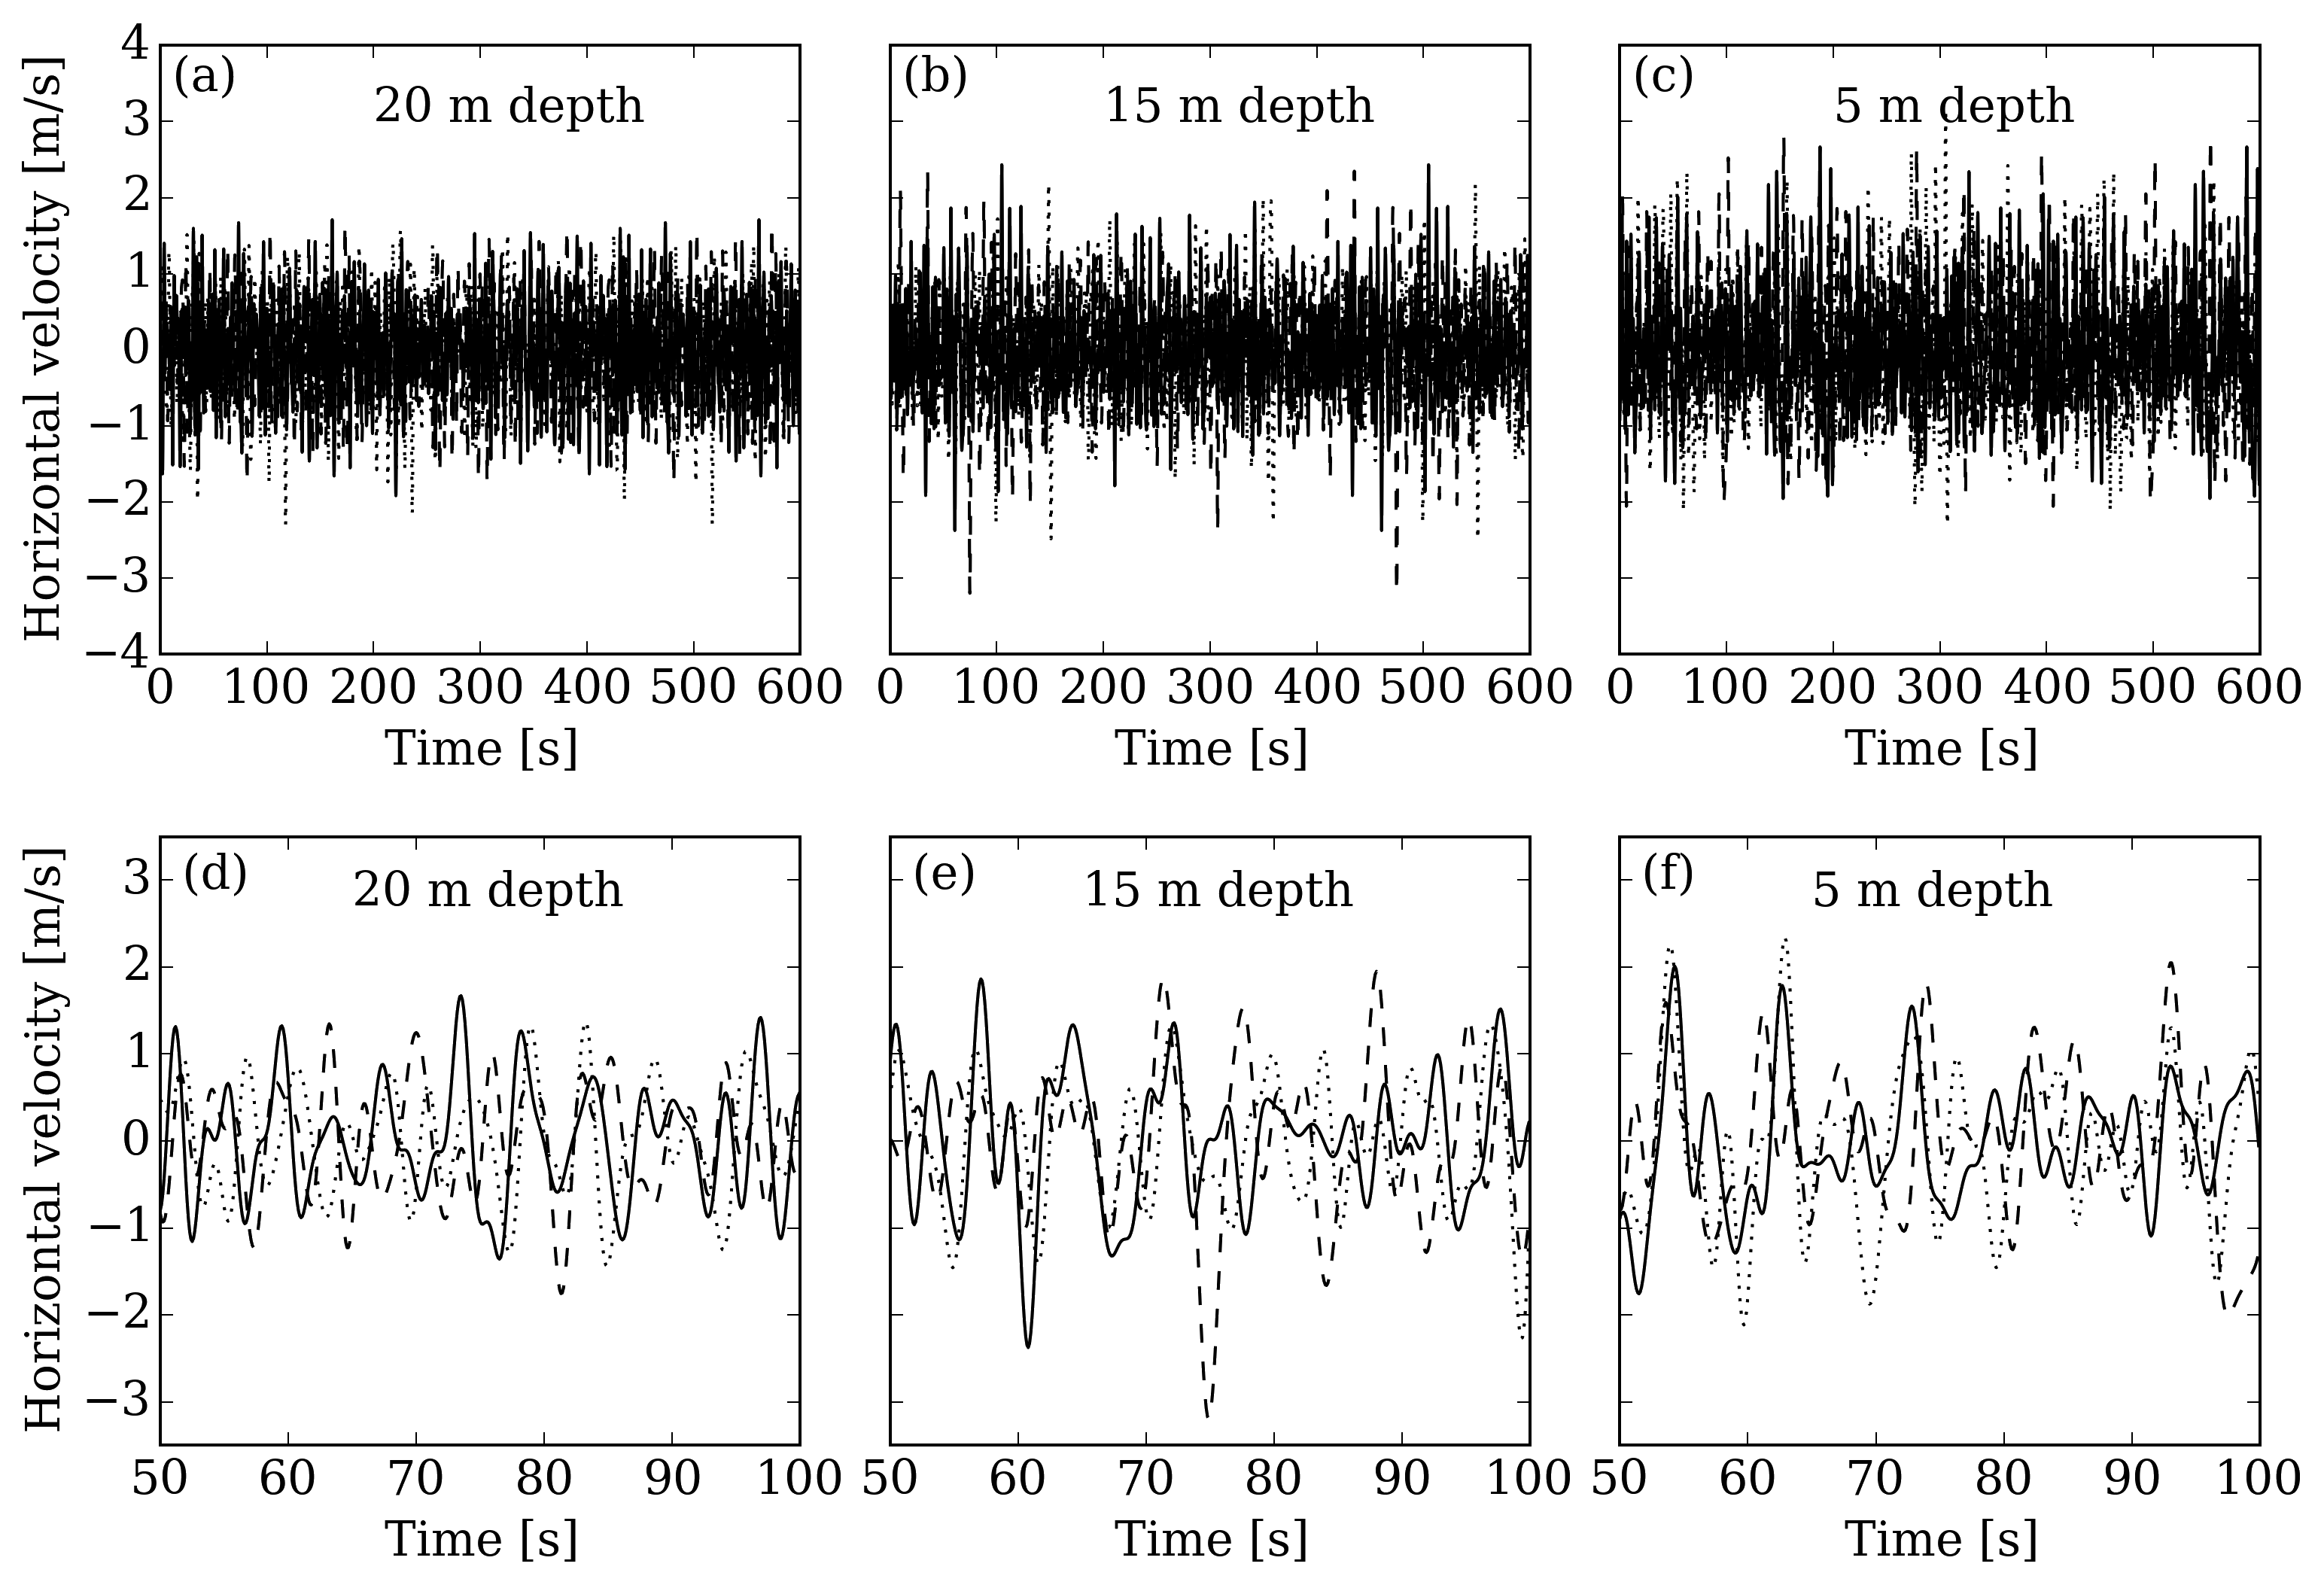
\includegraphics[scale=0.43]{WaveveloRealit.png}
\end{center}
\end{frame}

\begin{frame}[t]%{Boulder Dislodgement}
\begin{center}
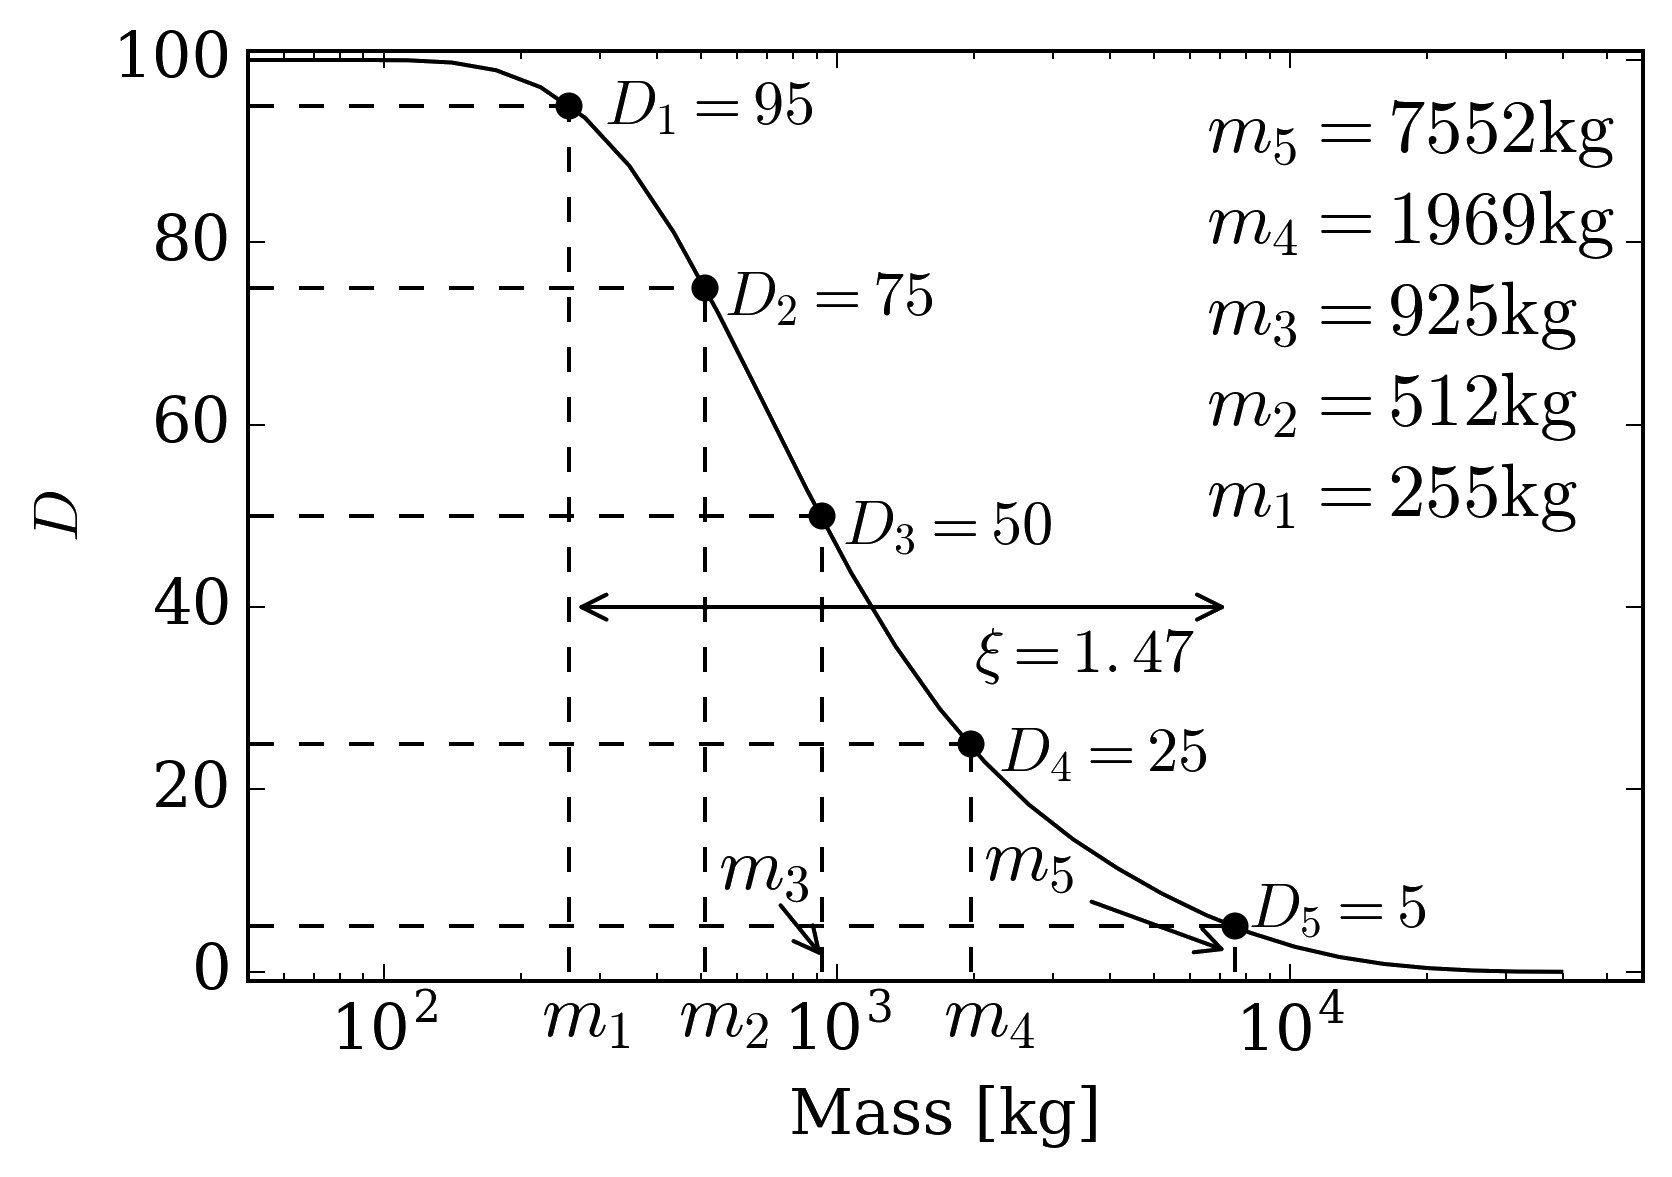
\includegraphics[scale=0.65]{dislodgmentexeedancet.png}

\vspace*{-1em}\begin{equation}
D=\frac{N_D}{N}
\end{equation}
$N$ is the total number of realizations ($N=100$), and $N_D$ is the number of
realizations for which boulder dislodgement occurred.
\end{center}
\end{frame}


\begin{frame}[t]%{Boulder Dislodgement}


\begin{picture}(1,6)
      \put(-25,-200){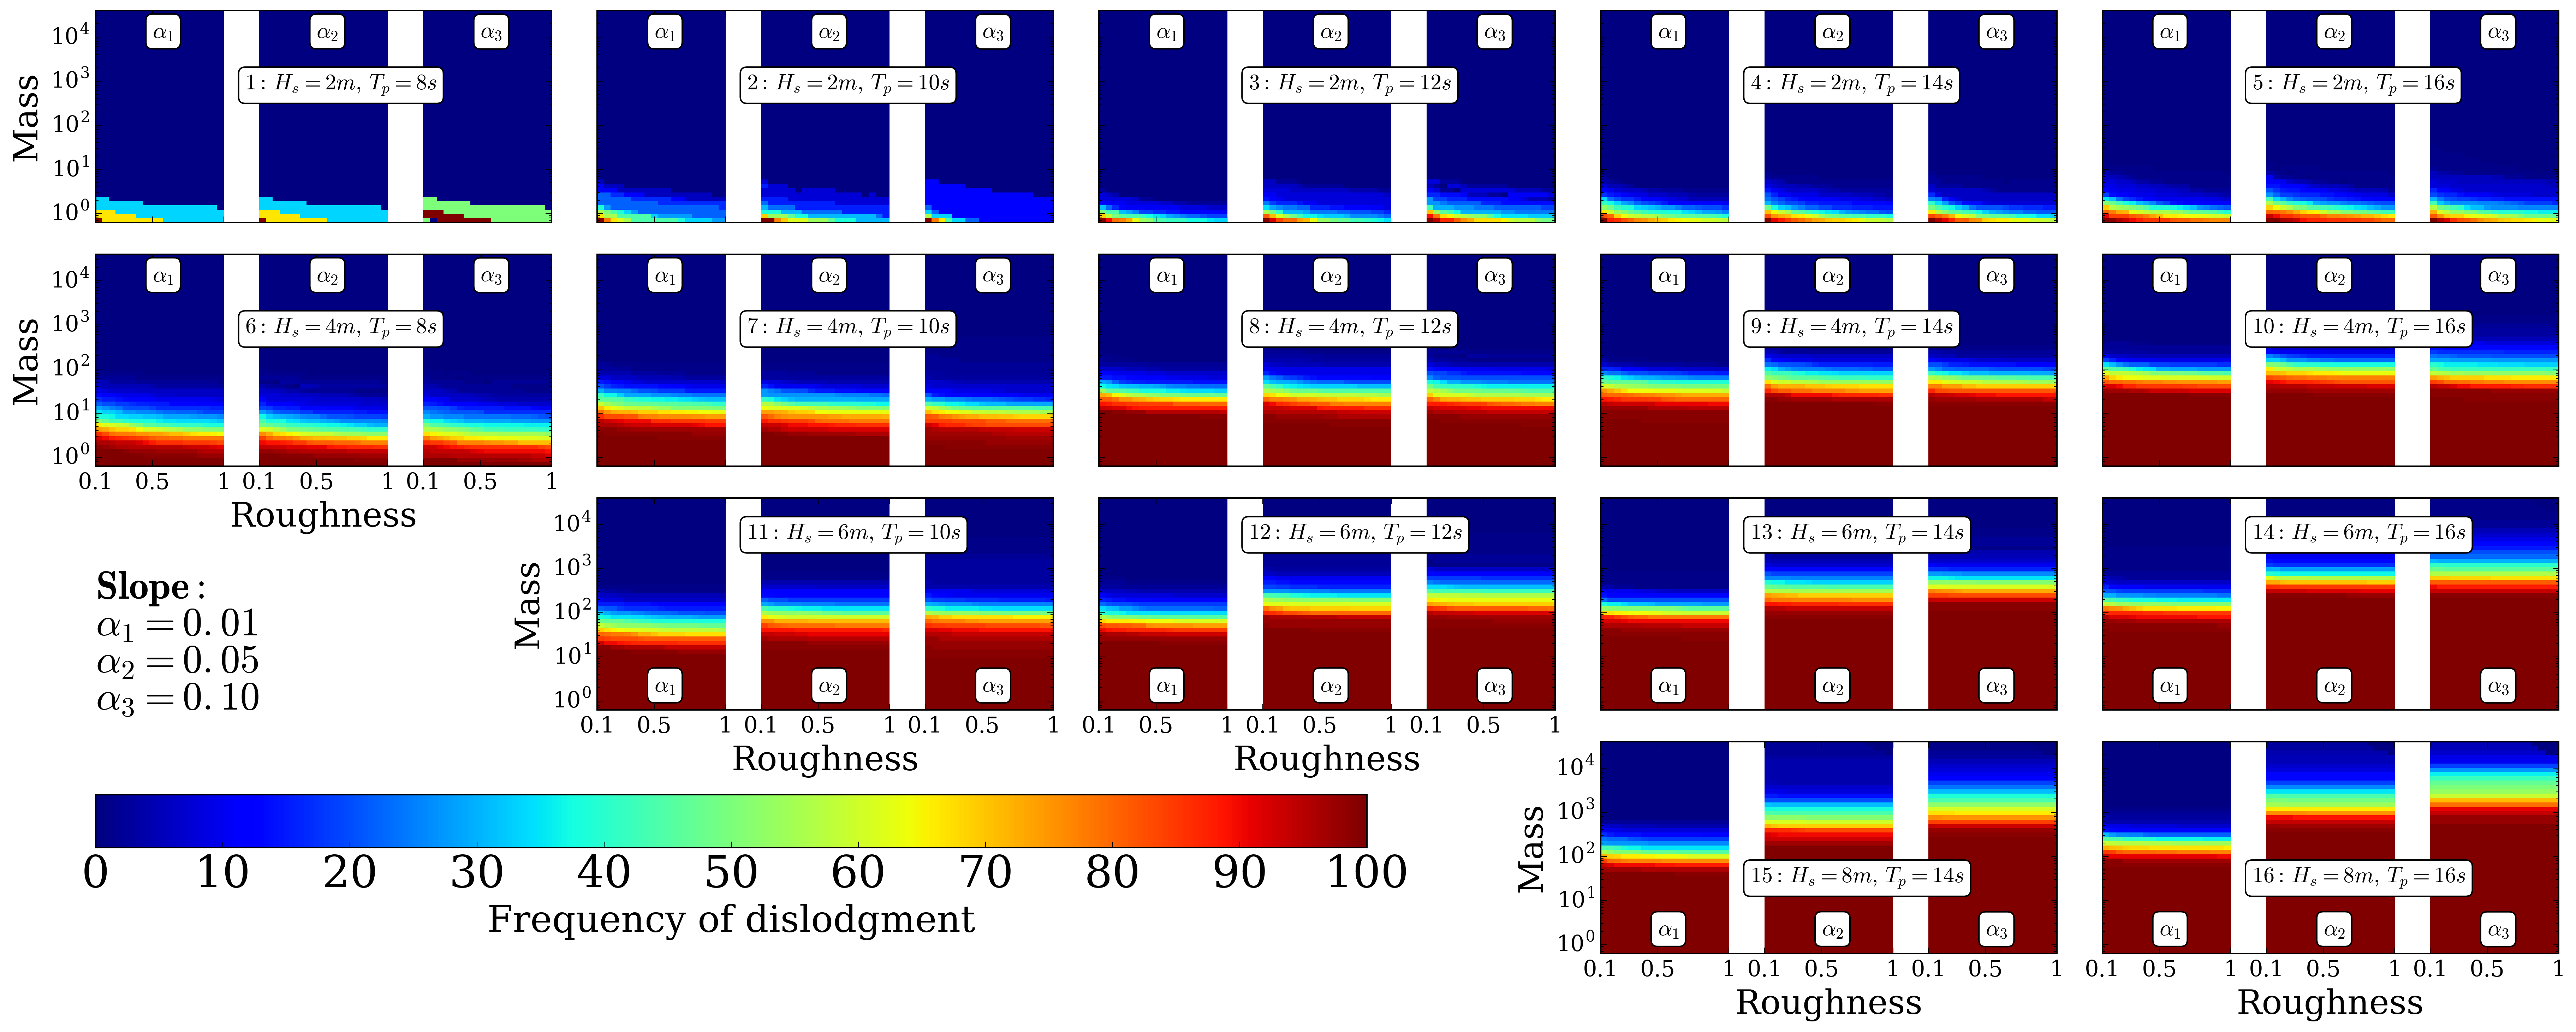
\includegraphics[scale=0.2]{ProbMapAllt.png}}
\end{picture}
\end{frame}

\begin{frame}[c]%{Boulder Dislodgement}

\begin{center}
Tsunami vs Storm

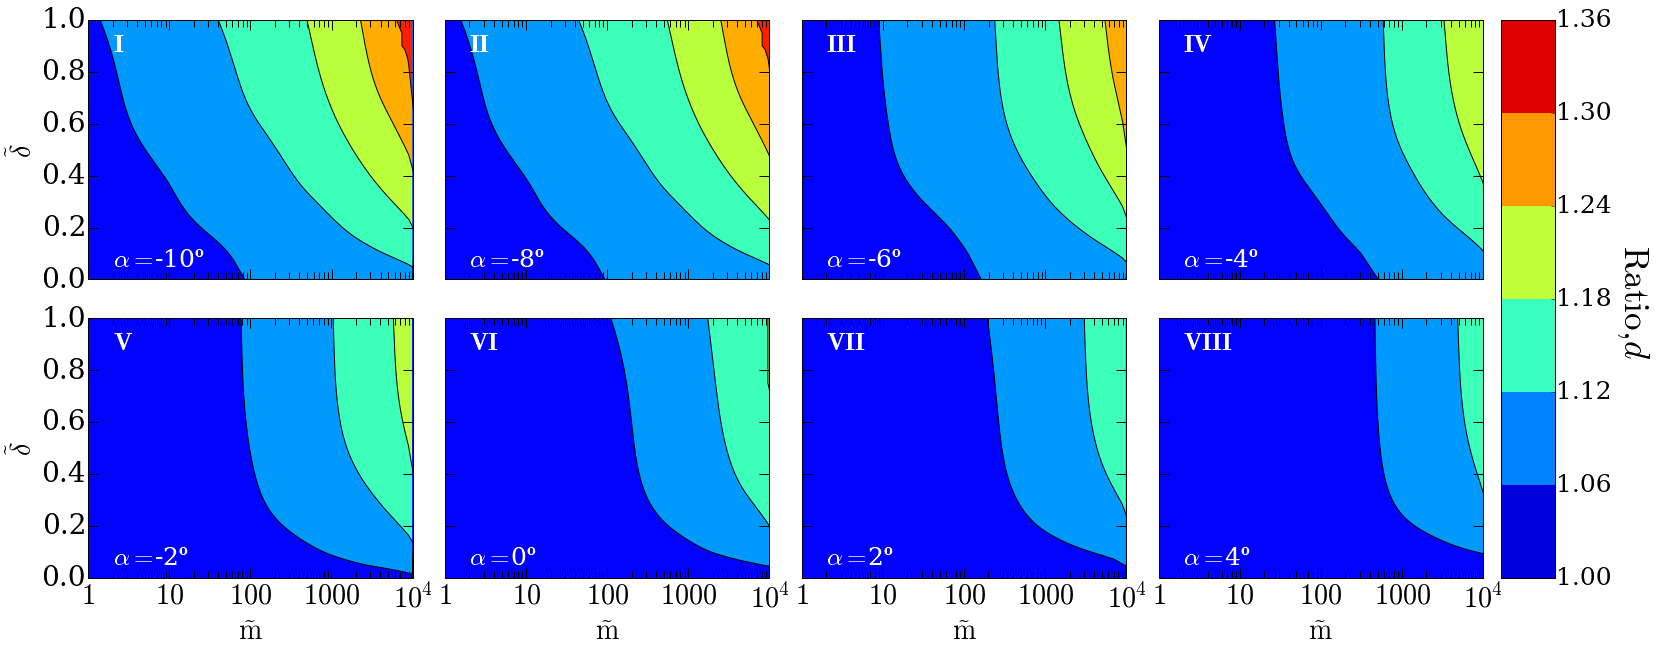
\includegraphics[scale=0.20]{testnew3t.png}
\end{center}
\end{frame}

\begin{frame}[t]

\begin{picture}(1,6)
      \put(-25,-200){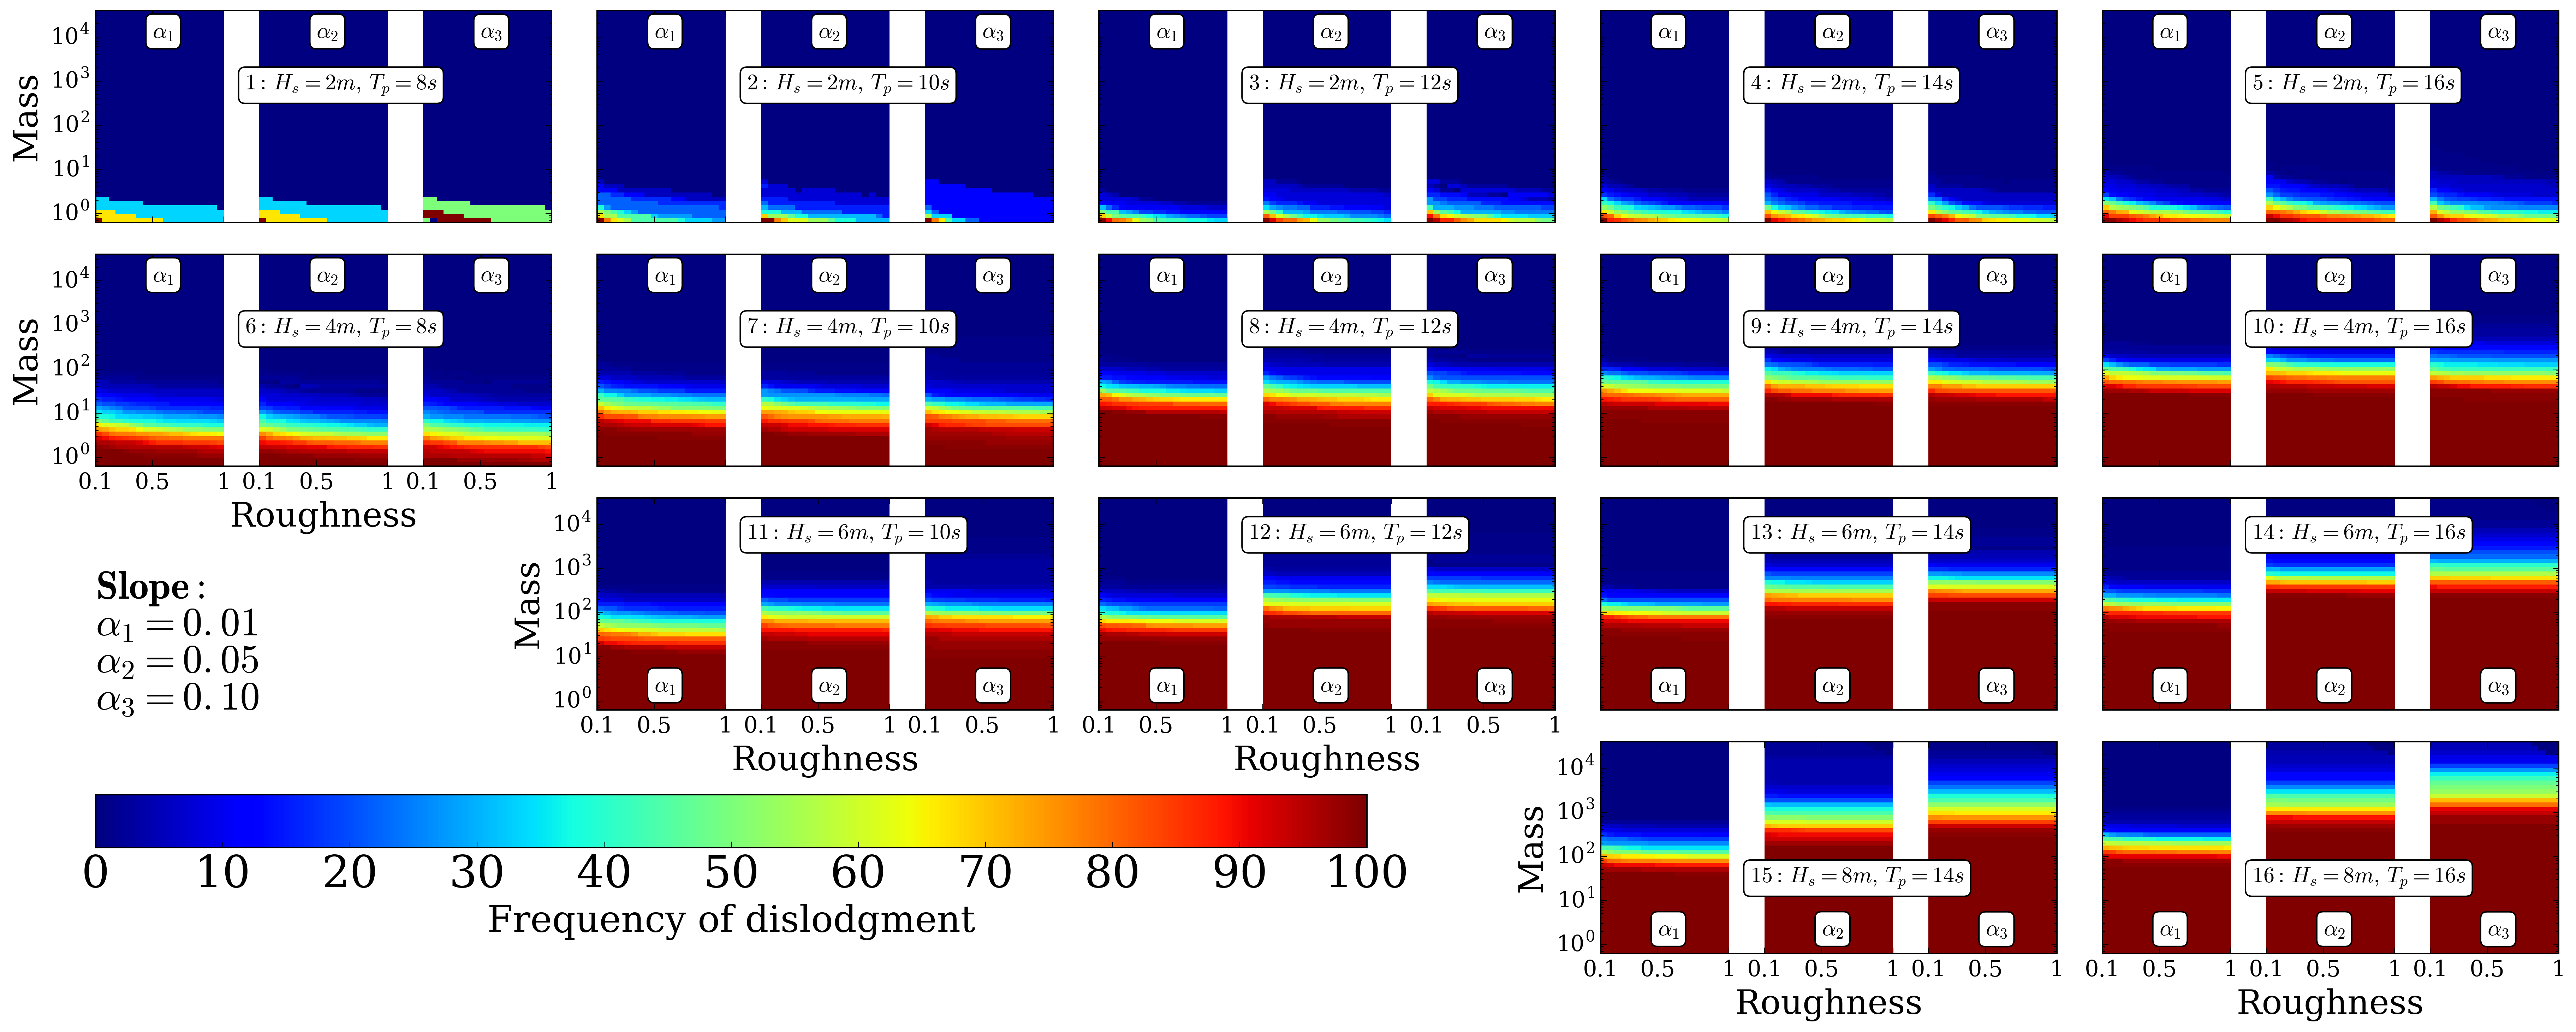
\includegraphics[scale=0.2]{ProbMapAllt.png}}
\end{picture}
\end{frame}



\begin{frame}[t]
\begin{center}

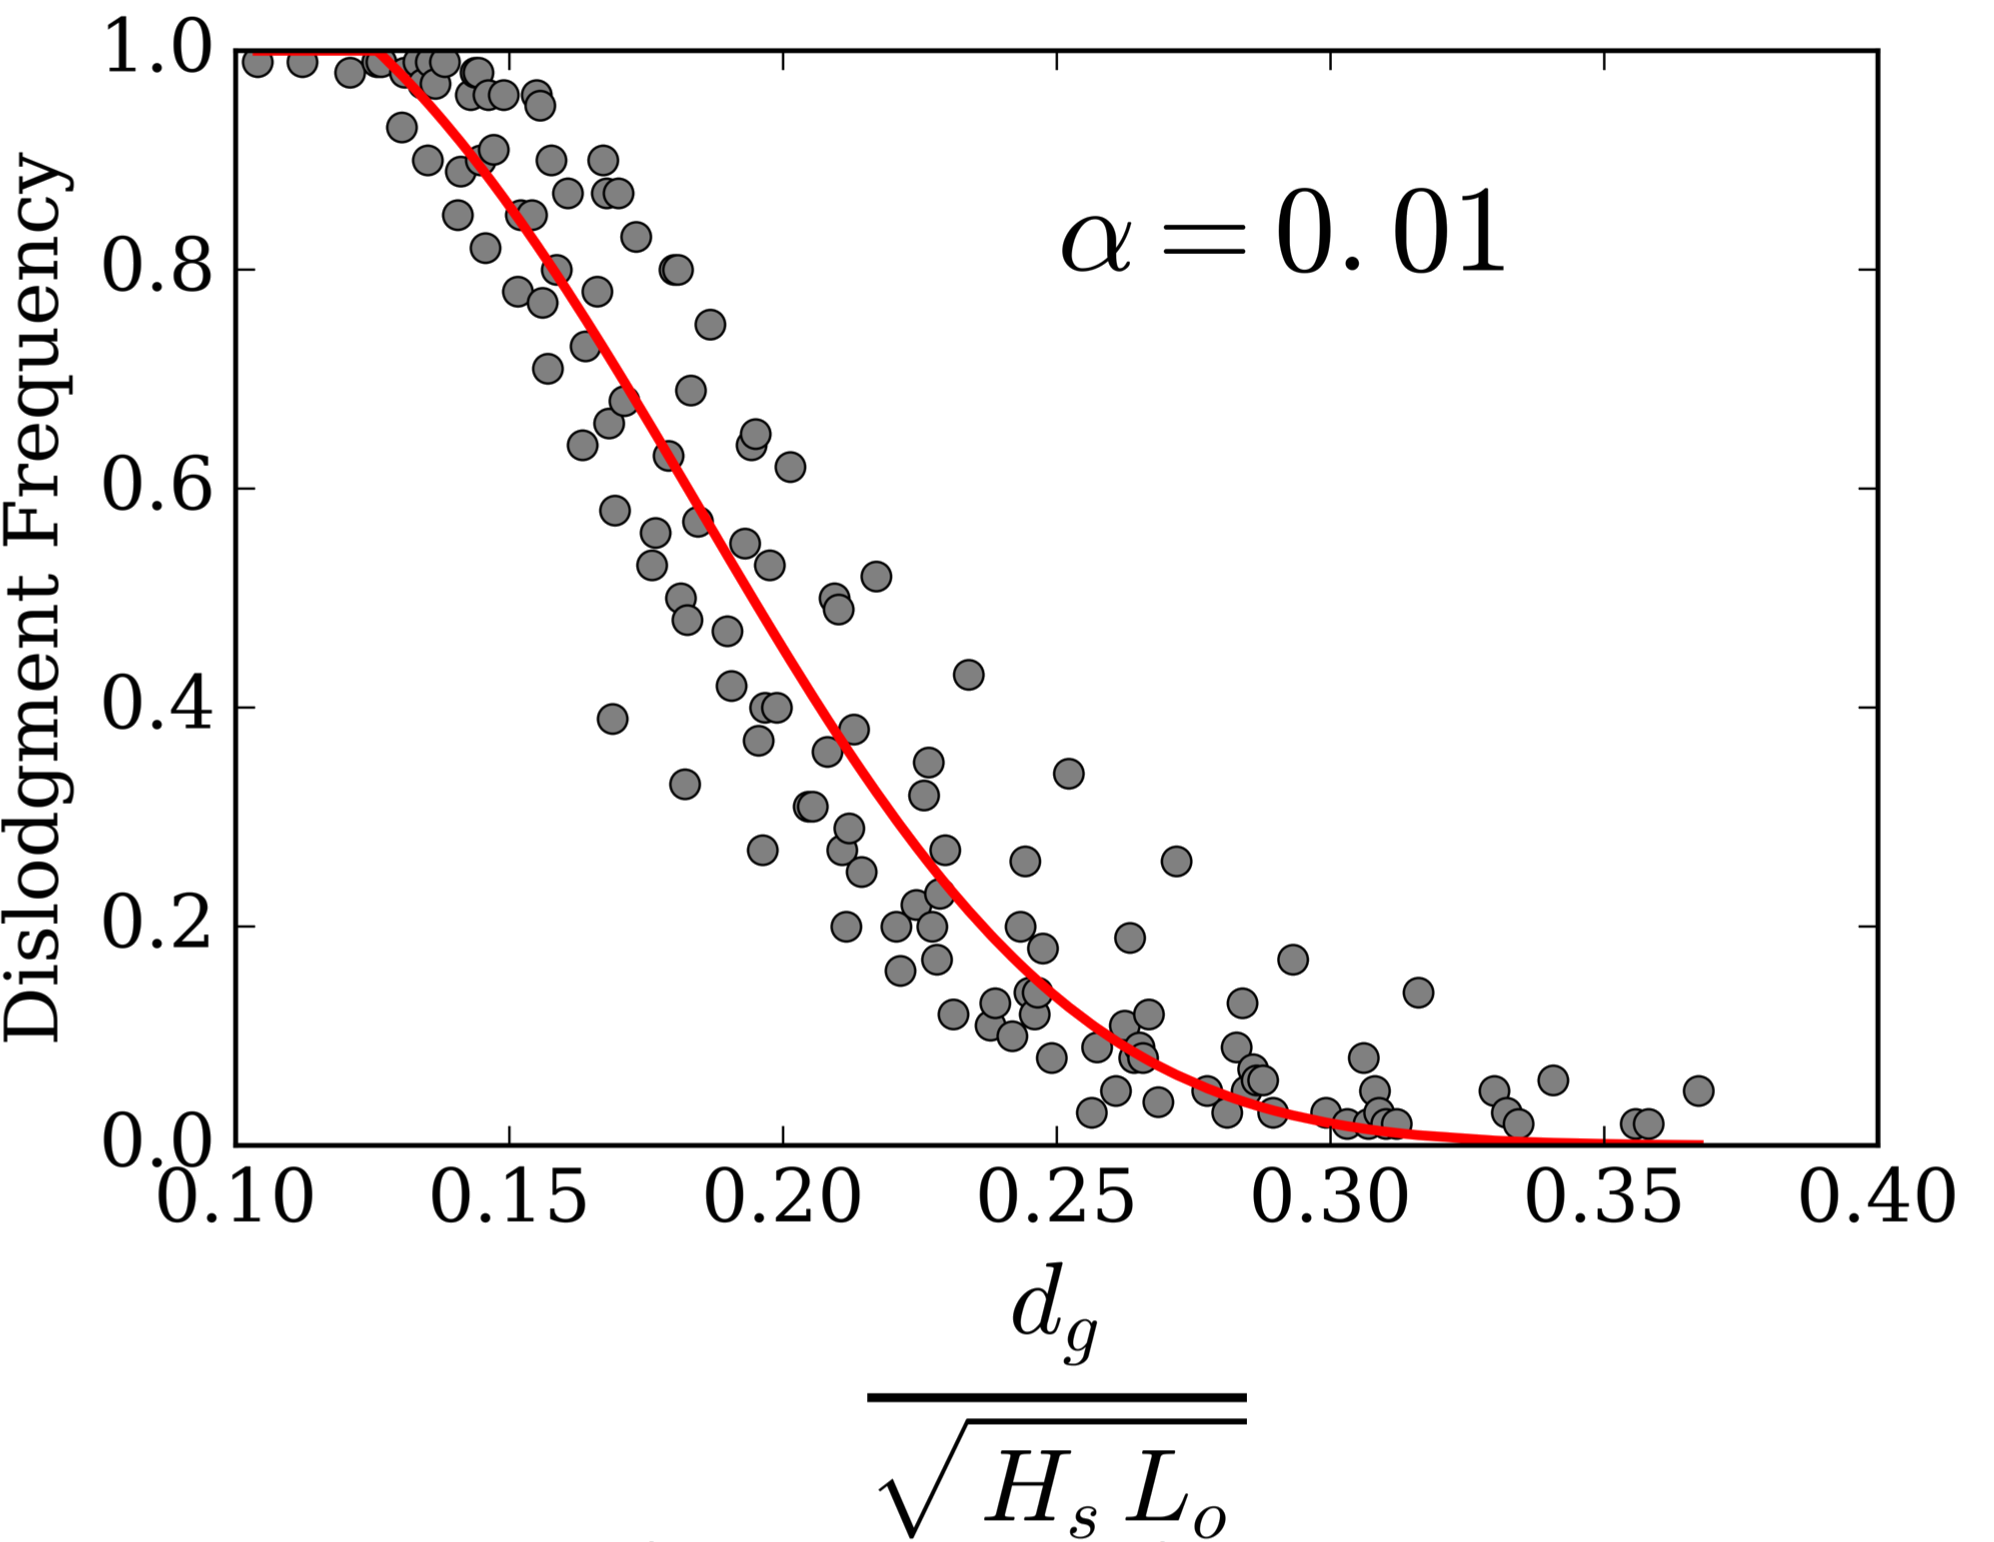
\includegraphics[scale=0.2]{bouldernewt.png}
\end{center}

\vspace*{-1em}\begin{equation}
H_s L_o = \frac{d^2_g}{2\alpha^2 \left[\textrm{erf}^{-1}(1 - 2D)\right]^2}
\end{equation}

From this and $L_o = 2\pi \;g \;T_p^2$, we can conclude that:
\begin{enumerate}
    \item $H_s \propto d^2_g$ and $T_p \propto d_g$
    \item $H_s \propto \left[\alpha^2\right]^{-1}$ and $T_p \propto \left[\alpha\right]^{-1}$
\end{enumerate}

\end{frame}



\end{document}
